% Escolha: Portugues ou Ingles ou Espanhol.
% Para a versão final do texto, após a defesa acrescente Final:

\documentclass[Ingles]{ic-tese-v1}
%\documentclass[Portugues,Final]{ic-tese-v3}

%\usepackage[latin1,utf8]{inputenc}
%\usepackage[portuguese]{babel}
\usepackage[utf8x]{inputenc}
% Para acrescentar comentários ao PDF descomente:
\usepackage
%  [pdfauthor={nome do autor},
%   pdftitle={titulo},
%   pdfkeywords={palavra-chave, palavra-chave},
%   pdfproducer={Latex with hyperref},
%   pdfcreator={pdflatex}]
{hyperref}


\usepackage[cmex10]{amsmath}
\usepackage[font=footnotesize,subrefformat=parens]{subfig}
\usepackage{tikz}
\usepackage{float}
\usepackage{subfig}
\usepackage{graphicx}
\usepackage{listings}
\usepackage{amssymb}
\usepackage{placeins}
\usepackage{multirow}
\usepackage{filecontents}
\usepackage{url}
%\usepackage[inline]{enumitem}
\usepackage{adjustbox}
\usepackage[cmex10]{amsmath}
\usepackage{adjustbox}
\usepackage{graphicx}
\usepackage{pifont}
\usepackage[justification=centering]{caption}
\usepackage{listings}
\usepackage{paralist}
\usepackage{url}
\usepackage{filecontents}
\usepackage{multirow}
\usepackage{array}
\usepackage{tabulary}
\usepackage{listings}
\usepackage{color}

\usepackage{footnote}
\makesavenoteenv{tabular}
\makesavenoteenv{table}

\definecolor{codegreen}{rgb}{0,0.6,0}
\definecolor{codegray}{rgb}{0.5,0.5,0.5}
\definecolor{codepurple}{rgb}{0.58,0,0.82}
\definecolor{backcolour}{rgb}{0.95,0.95,0.92}
\definecolor{darkblue}{rgb}{0.0,0.0,0.6}

\lstdefinestyle{mystyle}{
	backgroundcolor=\color{backcolour},
	commentstyle=\color{codegreen},
	numberstyle=\tiny\color{codegray},
	stringstyle=\color{codepurple},
 	basicstyle=\footnotesize,
	breakatwhitespace=false,
	breaklines=true,
	captionpos=t,
 	keepspaces=true,
	numbers=left,
	numbersep=5pt,
	showspaces=false,
	showstringspaces=false,
	showtabs=false,
	tabsize=2
}

\lstset{classoffset=0,
	   keywordstyle=\color{black},
           classoffset=1,
           morekeywords={__kernel, __global, __private},keywordstyle=\color{codepurple},
           classoffset=2,
           morekeywords={pragma,omp,parallel,target,map,data,device,for,simd,foreach,end,declare,scan},keywordstyle=\color{darkblue},
	   frame=single,
           style=mystyle
}

\floatstyle{ruled}
\newfloat{algoritmo}{thp}{loa}
\floatname{algoritmo}{Algoritmo}

% Colors on or off: Pick ONE
\newcommand{\ifColorText}[2]{\textcolor{#1}{#2}}  % Colors ON
%\renewcommand{\ifColorText}[2]{{#2}}                % Colors OFF

\newcommand{\REM}[1]{}

% To turn comments OFF simply comment out  the \Commentstrue line
\newif\ifComments

\Commentstrue

\ifComments
\newcommand{\chek}[1]{\noindent\textcolor{red}{Check: {#1}}}
\newcommand{\maicol}[1]{\noindent\textcolor{magenta}{Maicol: {#1}}}
\newcommand{\xavier}[1]{\noindent\textcolor{violet}{Matt: {#1}}}
\newcommand{\marcio}[1]{\textcolor{red}{ {#1}}}
\newcommand{\guido}[1]{\noindent\textcolor{magenta}{Guido: {#1}}}
\newcommand{\rem}[1]{\noindent\textcolor{gray}{Removed: {#1}}}
\newcommand{\new}[1]{\noindent\textcolor{blue}{ {#1}}}
\newcommand{\ed}[1]{\noindent\textcolor{red}{ {#1}}}
\newcommand{\short}[1]{\noindent\textcolor{blue}{ {#1}}}
\else
\newcommand{\chek}[1]{}
\newcommand{\maicol}[1]{}
\newcommand{\xavier}[1]{}
\newcommand{\marcio}[1]{}
\newcommand{\guido}[1]{}
\newcommand{\rem}[1]{}
\newcommand{\new}[1]{#1}
\newcommand{\ed}[1]{}
\newcommand{\short}[1]{}
\fi

% Additional new commands
\newcommand{\etal}{{\em et al. }}
\newcommand{\cL}{{\cal L}}
\newcommand{\map}{\texttt{map} }
\newcommand{\unmap}{\texttt{unmap} }
\newcommand{\rb}{\texttt{readBuffer} }
\newcommand{\rcap}[1]{Chapter~\ref{cap:#1}}
\newcommand{\rsec}[1]{Section~\ref{sec:#1}}
\newcommand{\rsecs}[2]{Sections~\ref{sec:#1} --~\ref{sec:#2}}
\newcommand{\rtab}[1]{Table~\ref{tab:#1}}
\newcommand{\rfig}[1]{Figure~\ref{fig:#1}}
\newcommand{\rfigs}[2]{Figures~\ref{fig:#1} --~\ref{fig:#2}}
\newcommand{\req}[1]{Equation~\ref{eq:#1}}
\newcommand{\reqs}[2]{Equations~\ref{eq:#1} --~\ref{eq:#2}}
\newcommand{\ttt}[1]{{\texttt{#1}}}
\newcommand{\tit}[1]{{\textit{#1}}}
\newcommand{\rfign}[3]{Figures~\ref{fig:#1}, \ref{fig:#2} \& \ref{fig:#3}}
\newcommand{\rlst}[1]{Listing~\ref{lst:#1}}
\newcommand{\rlsts}[2]{Listing~\ref{lst:#1}{#2}}
\newcommand{\rlstn}[3]{Listings~\ref{lst:#1}{#2}~--~\ref{lst:#1}{#3}}

\newcommand{\mat}[1]{${#1}$}
\newcommand{\bb}[1]{{\texttt{B#1}}}
\newcommand{\R}{\texttt{R}}
\newcommand{\W}{\texttt{W}}
\newcommand{\RW}{\texttt{RW}}
\newcommand{\X}{\texttt{X}}
\newcommand{\RWX}{\texttt{[R,W,RW]}}
\newcommand{\CPU}{\texttt{CPU}}
\newcommand{\GPU}{\texttt{GPU}}
\newcommand{\CG}{\texttt{[CPU,GPU,X]}}
\newcommand{\atup}[1]{\texttt{({#1})}}
\newcommand{\egen}[1]{$GEN[#1]$}
\newcommand{\ekill}[1]{$KILL[#1]$}
\newcommand{\ein}[1]{$IN[#1]$}
\newcommand{\eout}[1]{$OUT[#1]$}
\newcommand{\ca}[1]{\ttt{CA = #1}}
\newcommand{\aclang}{\textit{ACLang}}

\newcommand*\circled[1]{\tikz[baseline=(char.base)]{
		\node[shape=circle,draw,inner sep=1pt] (char) {#1};}}
\newcommand{\dc}{\underline{{ }{ }{ }} }

\usepackage{MnSymbol}


\begin{document}
% Escolha entre autor ou autora:
\autor{Eder Maicol Gomez Zegarra}
%\autora{Nome da Autora}

% Sempre deve haver um título em português:
\titulo{Suporte de Parallel Scan em OpenMP}

% Se a língua for o inglês ou o espanhol defina:
\title{Support for Parallel Scan in OpenMP}

% Escolha entre orientador ou orientadora. Inclua os títulos acadêmicos:
\orientador{Prof. Dr. Guido Costa Souza de Araujo}
%\orientadora{Profa. Dra. Nome da Orientadora}

% Escolha entre coorientador ou coorientadora, se houver.  Inclua os títulos acadêmicos:
\coorientador{Dr. Marcio Machado Pereira}
%\coorientadora{Prof. Dra. Eng. Lic. Nome da Co-Orientadora}

% Escolha entre mestrado ou doutorado:
\mestrado
%\doutorado



% Se houve cotutela, defina:
%\cotutela{Universidade Nova de Plutão}

\datadadefesa{24}{04}{2018}

% Para a versão final defina:
\avaliadorA{Prof. Dr. Guido Costa Souza de Araujo (Supervisor/\textit{Orientador})}{IC/UNICAMP}
\avaliadorB{Prof. Dr. Renato Ant\^{o}nio Celso Ferreira}{Universidade Federal de Minas Gerais (UFMG)}
\avaliadorC{Prof. Dr. Guilherme Pimentel Telles}{Institute of Computing - UNICAMP}

\finalversiontrue


% Para incluir a ficha catalográfica em PDF na versão final, descomente e ajuste:
%\fichacatalografica{Ficha-Catalografica-Protocolo-263947185.pdf}


% Este comando deve ficar aqui:
\paginasiniciais


% Se houver dedicatória, descomente:
%\prefacesection{Dedicatória}
%A dedicatória deve ocupar uma única página.


% Se houver epígrafe, descomente e edite:
% \begin{epigrafe}
% {\it
% Vita brevis,\\
% ars longa,\\
% occasio praeceps,\\
% experimentum periculosum,\\
% iudicium difficile.}
%
% \hfill (Hippocrates)
% \end{epigrafe}


% Agradecimentos ou Acknowledgements ou Agradecimientos
\prefacesection{Agradecimentos}

% Sempre deve haver um resumo em português:
\begin{resumo}
Prefix Scan (ou simplesmente scan) é um operador que computa todas as somas
parciais de um vetor. A operação scan retorna um vetor onde cada elemento é a
soma de todos os elementos precedentes até a posição correspondente. Scan é uma
operação fundamental para muitos problemas relevantes, tais como: algoritmos de
ordenação, análises léxicas, comparação de cadeias de caracteres, filtragem de
imagens, entre outros. Embora existam bibliotecas que fornecem versões
paralelizadas de scan em CUDA e OpenCL, não existe uma implementação paralela
do operador scan em OpenMP. Este trabalho propõe uma nova clausula que permite
o uso automático do scan paralelo. Ao usar a cláusula proposta, um programador
pode reduzir consideravelmente a complexidade dos algoritmos, permitindo que
ele concentre a atenção no problema, não em aprender novos modelos de
programação paralela ou linguagens de programação. Scan foi projetado em ACLang
(\texttt{www.aclang.org}), um framework de código aberto baseado no compilador
LLVM/Clang, que recentemente implementou o OpenMP 4.X Accelerator Programming
Model. Aclang converte regiões do programa de OpenMP 4.X para OpenCL.
Experimentos com um conjunto de algoritmos baseados em Scan foram executados
nas GPUs da NVIDIA, Intel e ARM, e mostraram que o desempenho da proposta da
clausula OpenMP é equivalente ao alcançado pela biblioteca de OpenCL, mas com a
vantagem de uma menor complexidade para escrever o código.
\end{resumo}

% Sempre deve haver um abstract:
\begin{abstract}
  Prefix Scan  (or simply scan) is  an operator that computes  all the
  partial sums of a vector. A scan operation results in a vector where
  each element  is the sum of  the preceding elements in  the original
  vector up to the corresponding position.  Scan is a key operation in
  many  relevant  problems  like  sorting,  lexical  analysis,  string
  comparison,  image  filtering  among   others.  Although  there  are
  libraries  that provide  hand-parallelized  implementations  of the scan
  in  CUDA and OpenCL,  no automatic parallelization solution exists
  for this operator in  OpenMP. This work proposes a new  clause
  to OpenMP which  enables  the  automatic synthesis of the
  parallel  scan.  By   using  the  proposed  clause   a  programmer  can
  considerably  reduce   the  complexity   of  designing   scan  based
  algorithms, thus allowing he/she to focus the attention on the problem
  and not on  learning new  parallel  programming  models  or
  languages.  Scan was designed  in AClang (\texttt{www.aclang.org}),
  an open-source LLVM/Clang compiler  framework     that  implements  the
  recently released OpenMP 4.X Accelerator Programming Model.
  AClang automatically converts OpenMP 4.X annotated program regions
  to OpenCL. Experiments running a  set of typical scan  based  algorithms
  on NVIDIA, Intel, and ARM GPUs reveal that  the performance
  of  the  proposed  OpenMP  clause  is equivalent to that achieved when using
  OpenCL library calls, with the advantage of  a
  simpler programming  complexity.
\end{abstract}


% Se houver um resumo em espanhol, descomente:
%\begin{resumen}
% A mesma regra aplica-se.
%\end{resumen}


% A lista de figuras é opcional:
\listoffigures

% A lista de tabelas é opcional:
%\listoftables

% A lista de abreviações e siglas é opcional:
% \prefacesection{Lista de Abreviações e Siglas}

% A lista de símbolos é opcional:
% \prefacesection{Lista de Símbolos}

% Quem usa o pacote nomencl pode incluir:
%\renewcommand{\nomname}{Lista de Abreviações e Siglas}
%\printnomenclature[3cm]


% O sumário vem aqui:
\tableofcontents


% E esta linha deve ficar bem aqui:
\fimdaspaginasiniciais


% O corpo da dissertação ou tese começa aqui:
\chapter{Introduction}
\label{cap:Introduction}

Parallelizing loops  is a  well-known research  problem that  has been
extensively  studied. The  most common  approach to  this problem  uses
DOALL~\cite{Lamport:1974} algorithms  to parallelize
the iterations of  loops which do not  have loop-carried dependencies.
Although  there  are   approaches  such  as  DOACROSS~\cite{doacross},
DSWP~\cite{Rangan:2004} and  BDX~\cite{Cesar:2015} that
can be  used to parallelize loop-carried dependent  loops, these algorithms
can  not  be  directly  applied   to  loops  that  are  sequential  in
nature. One  example of such loop  can found in the  implementation of
the scan operation.

Cumulative     sum,     inclusive     scan,     or     simply     {\it
	scan}~\cite{ScanAsPrimitive} is  a key operation that  has for goal
to compute  the partial  sums of  the elements of  a vector.  The scan
operation results in a new vector where each element is the sum of the
preceding  elements  of  the  input vector  up  to  its  corresponding
position. Scan is a central operation in many  relevant  problems  like  sorting,
lexical  analysis,  string comparison,  image  filtering, stream compaction,
histogram construction as well as  in many data
structure transformations~\cite{BlellochTR90}.

Scan  is a very simple  operation  that can  be generalized
in two flavors (\textit{inclusive} and \textit{exclusive}) as follows.
Given  a binary  associative  operator\  $\oplus$ and  a
vector of  n elements\ $x = [x_{0},  x_{1}, ...  ,x_{n-1}]$,
an   {\em    inclusive   scan}    produces   the    vector
$y =  [ x_{0}, x_{0}  \oplus x_{1},  ... ,x_{0} \oplus  x_{1} \oplus
... \oplus x_{n-1}]$.

\begin{figure}[t]
	\lstset{basicstyle=\scriptsize}
	\begin{lstlisting}[label=lst:PrefixSum, caption={The prefix sum implementation}, escapeinside={(*}{*)}]
	(a) Sequential implementation

	y[0] = 0;
	for(int i = 1; i < n; i++)
		y[i] = y[i-1] + x[i-1];

	(b) Parallel implementation using the new clause

	y[0] = 0;
	#pragma omp parallel for scan(+: y)
	for(int i = 1; i < n; i++)
		y[i] = y[i-1] + x[i-1];
	\end{lstlisting}
	\vspace{-0.7cm}
\end{figure}

\begin{eqnarray}
y[0] = 0\nonumber\\
y[1] = x[0] \nonumber\\
y[2] = x[0] + x[1] \nonumber\\
y[3] = x[0] + x[1] + x[2] \nonumber\\
\dots\nonumber\\
y[i] = \sum_{j=0}^{i-1} x[j]
\label{eq:scan}
\end{eqnarray}

Similarly,  the  {\em  exclusive  scan} operation  results  in  vector
$y =  [ I, x_{0}, x_{0}  \oplus x_{1}, ... ,x_{0}  \oplus x_{1} \oplus
... \oplus x_{n-2}]$, where $I$ is  the identity element in the binary
associative operator  $\oplus$. The  parallel scan clause  proposed in
this work  is based  on the  exclusive scan  operation which  will be
called \textit{scan} from now on.   It is trivial to compute inclusive
scan from  the result of its  exclusive version. This can  be done by:
(i) computing the exclusive scan of $y$; (ii) shifting the elements of
$y$    to    the   left;    and    (iii)    storing   the    operation
$y[n-2] \oplus x[n-1]$ into $y[n-1]$.

The scan of a sequence is trivial to compute using an $\mathcal{O}(n)$
algorithm   that   sequentially   applies   the   recurrence   formula
$y[i]  = y[i-1]  \oplus  x[i-1]$  to the  $n$  elements  of $x$.   For
example,   when  the   binary  operator   $\oplus$  is   the  addition
(\req{scan}), the  scan operation  stores in $y$  all partial  sums of
array  $x$,  an algorithm  named  \textit{Prefix  Sum}.  As  shown  in
\rlsts{PrefixSum}{a}, the  loop   that  implements   prefix  sum   is
intrinsically  sequential due  to the  loop-carried dependence  on $y$
which makes the  value of $y[i]$ depend on the  value of $y[i-1]$ from
the previous  iteration. Hence,  the loop body  in \rlsts{PrefixSum}{a}
forms a  single \textit{strongly  connected component} in  the program
control-flow  graph~\cite{flowgraph} and  thus typical  DOACROSS based
algorithms like~\cite{926166,344315} cannot  be used  to parallelize
the loop iterations of prefix sum.

There are many  other scan based operations that use various
associative  binary  operators  like product,  maximum,  minimum,  and
logical  \texttt{AND}, \texttt{OR},  and  \texttt{XOR} to  parallelize
some                           very                           relevant
algorithms~\cite{NEEDLEMAN1970443,Crow:1984:STT:800031.808600,minimum}.
Given  the relevance  of  scan in  computing,  library based  parallel
implementations    of    scan    have    been    proposed    in    the
past~\cite{dataparallel,  ScanAsPrimitive}  and  designed  as  library
calls   in  languages   like   OpenCL  and   CUDA~\cite{Sengupta:2007,
	Capannini:2011}.   Unfortunately, most  of these  implementations are
problem specific leaving the programmer with the task of mastering the
complexity of OpenCL and CUDA in order  to handle the design of a scan
based operation to a specific problem.

This work proposes a new OpenMP \texttt{scan} clause that enables the
automatic synthesis of parallel  scan.  The programmer can
use the new  clause to  design algorithms in OpenMP C/C++ code
thus eliminating the need to deal with  the complexity of OpenCL or CUDA.
The  new   scan  clause   was  integrated  into   \textit{ACLang},  an
open-source LLVM/Clang compiler framework (www.aclang.org) that
implements  the  recently   released  \textit{OpenMP  4.X  Accelerator
	Programming   Model}~\cite{MPereira2017}.     AClang   automatically
converts OpenMP 4.X annotated program regions to OpenCL/SPIR kernels,
including those regions containing the new scan clause.


A careful  reader might think that  such new scan clause  is a trivial
extension of the  reduction clause already available in  OpenMP.  As a
matter of fact, the reduction of the elements of a sequence $x$ can be
obtained  by  computing  the  scan  of   $x$  into  $y$  as  shown  in
\rlsts{PrefixSum}{b} and returning the value of $y[n-1] + x[n-1]$.  In
other  words, reduction  is a  simpler version  of scan  in which  the
values of all intermediate partial sums  are not exposed, and only the
total  sum of  the  elements of  $x$ is  returned.   Reduction can  be
performed    in    $\mathcal{O}(log\    n)$   complexity    using    a
tree-based~\cite{tree-based}                    or                   a
butterfly-based~\cite{butterfly-based} parallel  algorithm.  Moreover,
both  reduction  and  scan  are operations  that  handle  loop-carried
dependent  variables.   In  the  reduction  case,  a  single  variable
accumulates the value from the  previous iterations, while in scan the
accumulation  occurs for  all  elements of  $y[i]$  each depending  on
elements from the previous  iterations.  This makes the implementation
of parallel scan much harder than the implementation of reduction.
The rest of the work is organized as follows. \rcap{background} details
some concepts of programming to GPU, and the AClang compiler. \rcap{Scan}
describes the state-of-art of the scan algorithm used to design and implement
the new OpenMP scan clause. Also, this Chapter gives an outline of the
structure of the AClang compiler and describes the details of the
implementation of the OpenMP scan clause into the AClang Compiler.
\rcap{ScanUse} describes some examples of the use of the scan clause.
\rcap{RelatedWorks} discusses related work, and \rcap{Experiments} provides
performance numbers and analyzes the results when programs are compiled with
the new scan clause. Finally, \rcap{Conclusion} concludes the work.

\chapter{Background}
\label{cap:background}

\section{Introduction to GPUs}
\subsection{A Brief History of GPUs}
In the early 1990s, users began purchasing
2D display accelerators for their computers. These display accelerators
offered hardware-assisted bitmap operations to assist in the display and usability
of graphical operating systems.

Around the same time, the company Silicon Graphics popularized the use
of three-dimensional graphics. In 1992, Silicon Graphics opened the
programming interface \rem{to}\new{for} its hardware\rem{ by releasing the OpenGL library they wanted
that OpenGL was used as a standardized.}\new{, launching the OpenGL library, so that it became a de facto standard.}

By the mid-1990s, the demand for applications that were using 3D graphics
increases considerably, growing one stage of development. PC gaming was affected
by those devices \rem{to create}\new{creating} progressively, more realistic 3D environments.
At the same time, companies such as NVIDIA, ATI Technologies,
and 3dfx Interactive, began releasing graphics accelerators that were affordable
enough to attract widespread attention. These developments cemented 3D
graphics as a technology that would \rem{figure}\new{become} prominent\rem{ly} for years to come.

In 1999 was created the first GPU GeForce 256 that was marketed as "the world's
first GPU" or Graphic Processing Unit, enhancing the potential
for even more visually interesting applications. Since transform and lighting were
already integral parts of the OpenGL graphics pipeline, the GeForce 256 marked
the beginning of a natural progression where increasingly more of the graphics
pipeline would be implemented directly on the graphics processor.

In 2001 was introduced the GeForce 3 that is the first programmable GPU that means
for the first time, developers had some control over the exact computations
that would be performed on their GPUs.

\subsection{GPU Overview}
Graphics processor units were designed to allow to handle massive computations
that are required to render the graphics that are created and displayed by a computer.
Commonly, this requires the execution of the same operation on a large data set. Insomuch as that processing should be in real time. it must be completed as
fast as can be done. The GPU was the answer to how to do this. A GPU consists of many cores. These all cores are capable of executing a thread.
Generally, each thread performs an operation on a sample data. This allows that the large data can be operated in parallel.
GPU was designed for graphics processing in mind, and this was the main application for GPUs
for a long time. Lately, researcher and programmers discovered a opportunity the ability of the GPUs for high levels of parallelization. This is becomes an opportunity to increase the performance of many general purpose programs.
That is how started what is known as general purpose graphics processing unit programming or GPGPU programming. With the steady growth interest in GPGPUs programming, GPU vendors started creating GPUs for different applications in mind, thus, the toolkit was created to allow programming in the GPUs. This toolkit, known as CUDA, allows the programmer to create applications that can run on GPUs. A major advantage of CUDA is its similarity with the C language. This allows the implementation of many applications as well as the increase in the number of parallel algorithms to harness the potential of the GPU. As was mentioned before, GPUs have the ability to execute a program in parallel. The downside to using GPU is the fact that a CPU is necessary mandatory. The GPU by itself can't be a standalone unit. To be able to operate on a GPU, the presence of the CPU is necessary to manage the execution of the program. The CPU is responsible for determining which portions of the application are completed by the GPU and what the parameters will be used in this operation. Also, an important function of the CPU is responsible for the memory management of the GPU. Thereby the operations are performed in the GPU, the data must be copied from the CPU memory. In the same way, when the GPU finished its work, it is necessary pass the data from the GPU to the CPU. This is a very expensive operation that often limits the programmers to be able to use the GPU.
In addition to the above explained the use of the GPU has several other disadvantages.
Similarly to the digital signal processor (DSP), the GPU has a slower clock speed than the CPU. It also does not have the same size of the cache. It does not implement branch prediction or any of that type of optimization. For this reason a GPU cannot keep up with the CPU in serial execution.
For these reasons, it is very important to define what portions of the program can be done serially and executed on the CPU, meanwhile what portions could be parallelized and executed on the GPU. If the proportion to be executed in the GPU compensates in time with all the disadvantages mentioned above and it is faster than its serial version, worth the use of the GPU.
There have been done many studies on the GPU and how is possible to use the GPU in several research areas. The new ease of use has also contributed to an increase in the number of people wanting to conduct research into the viability of a GPU implementation for their application. Studies also look at the various ways that the GPU can be utilized to improve performance. A very common situation nowadays is the waiting of many people for some research that makes possible the use of GPUs in their applications.
As an example, Trancoso \etal~\cite{Trancoso2005} analysed a very simple application as implemented on a GPU, a low-end CPU, and a high-end CPU. They discussed the application’s performance on the GPU relative to the CPU and also looked at several of the different variables that can be changed to improve the GPU’s performance. They also looked at what factors make a program more likely to be better suited for a GPU than a CPU.
Another example, Owens \etal~\cite{Owens2008}, they studied how the GPU can handle applications that were previously implemented on a CPU. That study looks at the GPU design and discusses about the possible performance improvements offered for the GPU. Also they analyzed how the GPU was used for specific applications such as in-game, physics and computational biophysics.

As CUDA was mentioned, it is also important to mention OpenCL. The OpenCL standard is the first open, royalty-free, unified programming model for accelerating algorithms on heterogeneous systems. OpenCL allows the use of a C-based programming language for developing code across different platforms, such as CPUs, GPUs, DSPs, and field-programmable gate arrays (FPGAs).
OpenCL is a programming model for software engineers and a methodology for system architects. It is based on standard ANSI C (C99) with extensions to extract parallelism. OpenCL also includes an application program interface (API) for the host to communicate with the hardware accelerator (mainly GPU), traditionally over PCI Express, or one kernel to communicate with another without host interaction.
In the OpenCL model, the user schedules tasks to command queues, of which there is at least one for each device. The OpenCL run-time then breaks the data-parallel tasks into pieces and sends them to the processing elements in the device. This is the method for a host to communicate with any hardware accelerator. It is up to the individual hardware accelerator vendors to abstract away the vendor-specific implementation.
Summing up what was said before, OpenCL is an framework that allows the use of several devices from different vendors. So many developers agree that CUDA has a better performance than OpenCL in Nvidia devices however, no all the costumers have Nvidia card therefore in several times is preferred OpenCL instead of CUDA. Clearly if Nvidia card is a option, CUDA will always be chosen.

\subsection{GPU hardware}
\label{sec:gpugardware}
Before going into the programming of GPUs (see~\rsec{gpuprogramming}), it is important to have some background \rem{about}\new{in} GPU architecture.
The GPU programming model exposed by CUDA very much mirrors the underlying
hardware. Some of the details that make GPU programming hard are more apparent
when looking at the underlying hardware.
A CUDA GPU is built around a single kind of processor (as opposed to the different
kinds of processors found in earlier GPUs). The processors in the GPU (called
MPs, MultiProcessors) all contain a number of cores called SPs (Streaming Processors).
Each MP also contains local memory, called shared memory since it can be
accessed by all of the SPs in that MP. The number of MPs varies over the available
GPUs; cheaper GPUs have as few as one MP, and as you go up in price the number
of MPs increases.
Each MP of the GPU can manage a large number of threads; on today’s GPUs
up to 2048 threads can run on a single MP. The GPU schedules threads in groups
of 32, called Warps, that are executed in lock-step (SIMD style execution). Threads are also divided into Blocks; the threads within a block can communicate using the
shared memory. The maximum number of threads per block is 1024 ~\cite{NvidiaGuide2018}. Threads within
a warp can communicate via the shared memory without using any synchronisation
primitive. However, if communication takes place across warps synchronization is
necessary. A barrier synchronization mechanism exists to ensure that all threads
within a block have reached the same position in the code. Blocks are also grouped
into a grid, that is the collection of blocks executing the same program.

\subsection{Programming for GPUs}
\label{sec:gpuprogramming}
The GPGPU programming landscape has rapidly evolved over the past several years. This allowed that in these days there are several approaches to programming GPUs. For this section, CUDA language will be taken as a reference.

CUDA is a parallel computing platform and programming model developed by NVIDIA designed for GPU computing.
CUDA computing system has two parts: The host and device.
The host part is one or many traditional CPU(s) like Intel or AMD CPUs. The
device part is consist of one or several GPU(s), which is used as co-processors. Since
GPU can involve a lot of parallelisms, CUDA devices could help to accelerate those applications that have a lot of data to  parallelize. Thus, parallelism is the key factor to decide if the application is appropriate for a CPU-GPU system.

\subsubsection{CUDA Function Declaration}
\label{CUDAfunction}

As stated above, a complete CUDA Program is a mixed code with both GPU and CPU
code. Function declaration keywords is designed to support this kind of mix coding. As
shown in \marcio{Não seria Table ??} \rem{Fig.4.1, functions in CUDA is declared as global, host and device.}\new{functions in CUDA can be declared as global, host or device.} A kernel
function is the function that will generate a large number threads and it is declared as
global. During the compilation, the NVCC compiler will generate thousands \new{of} threads for
the kernel function and map them to the GPU. \new{The keyword} device is used to declare a CUDA device
functions that can only be executed on GPU. In addition, a CUDA device function can
only be called in a kernel function. The last keyword, host, is design for declaration for a
host function which is run on CPU. \new{The keywords} host and device can be used \rem{to} together to instruct
the compiler to generate two versions \rem{for both GPU and CPU.}\new{of the kernel, one to running on CPU and another for the GPU.}


\begin{center}
	\begin{tabular}{ | c | >{\centering\arraybackslash}p{2cm} | >{\centering\arraybackslash}p{3cm} |}
		\hline
		 & Executed on the: & Only callable from the: \\ \hline
		{\color{blue} \_device\_} int DeviceFunction() & device & device \\ \hline
		{\color{blue} \_global\_} void KernelFunction()& host & device \\ \hline
		{\color{blue} \_host\_} int HostFunction() & host & host\\
		\hline
	\end{tabular}
\end{center}

\subsubsection{CUDA Thread Organization}
\label{CUDA Thread Organization}
When a kernel is executed, the execution is distributed over a grid of thread
blocks as \rem{illustrated below}\new{shown} in \rfig{threadsblocks}. Since all \rem{the} threads are executed in the kernel function, \rem{there should be some mechanisms to help to distinguish themselves and know what area of data they should work on.}\new{some mechanisms are necessary to define in which data area the threads must work.} In CUDA, all threads are organized in two-level hierarchy-block and grid, as shown in \rfig{threadorganization}. A number of threads compose a block and uses the threadIdx to index them in a block. A grid is organized in the same way and uses blockIdx to index each block in a grid. Both threadIdx and blockIdx are pre-defined variables of CUDA. In addition, there are another two pre-defined variables blockDim and gridDim, which are used to indicate the dimension block and grid by number of threads in a block and number of blocks in a grid. An example is showed in \ref{fig:cudaindex}.

\begin{figure}[t]
	\centering
	\caption{A two-dimensional arrangement of 8 thread blocks within a grid.}
	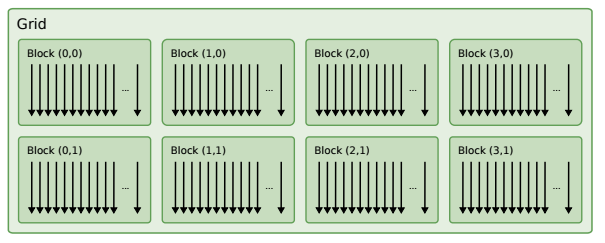
\includegraphics[scale=0.70]{images/threadsblock.png}
	\label{fig:threadsblocks}
\end{figure}

\begin{figure}[t]
	\centering
	\caption{CUDA Thread Organization}
	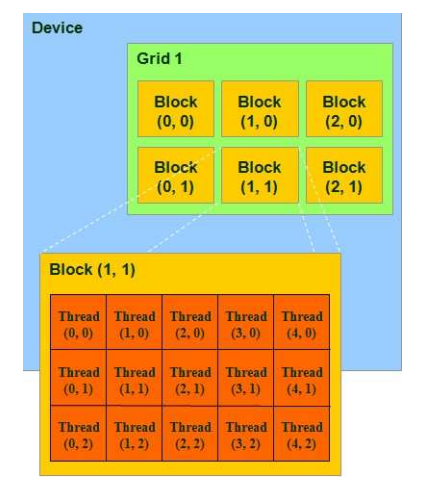
\includegraphics[scale=0.70]{images/thread_organization.png}
	\label{fig:threadorganization}
\end{figure}

\begin{figure}[t]
	\caption{CUDA parallel thread hierarchy}
	\centering
	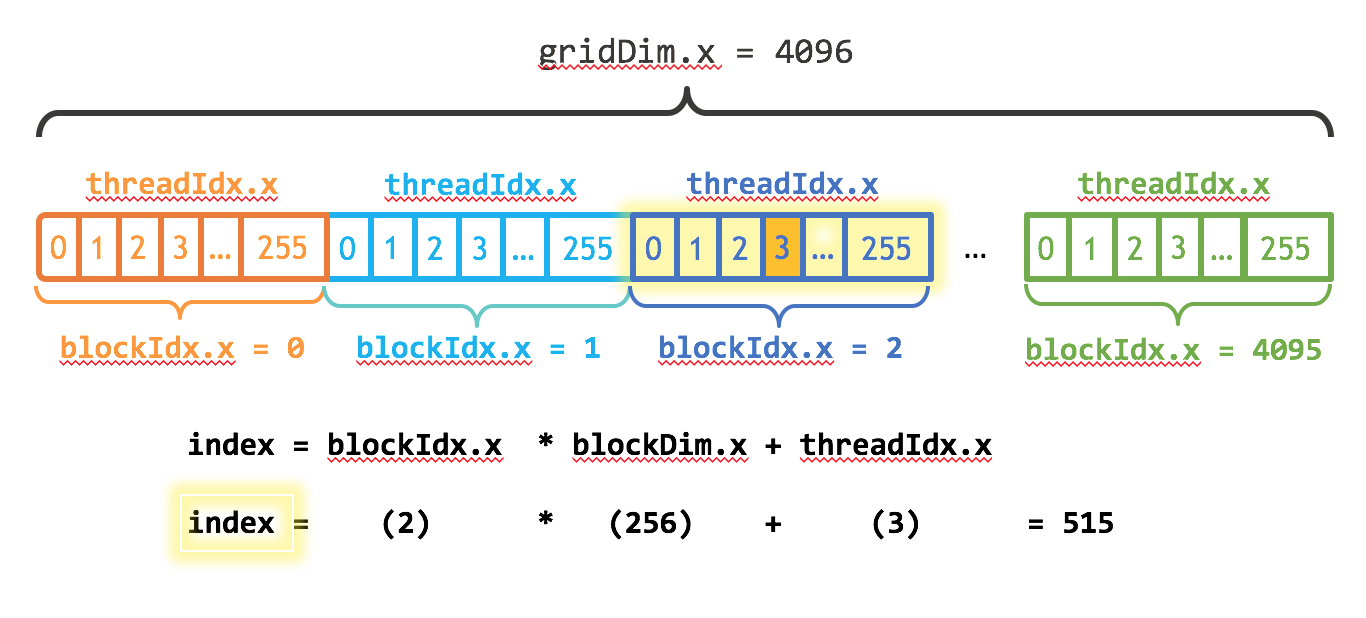
\includegraphics[scale=0.60]{images/cuda_indexing.png}
	\label{fig:cudaindex}
\end{figure}

\subsubsection{CUDA Device Memory}
\label{CUDA Device Memory}
Memory hierarchy is one of the main factors in a system. \rfig{cudamemory} shows the overview of the CUDA memory hierarchy. Exists four kinds of memory in CUDA: global
memory, constant memory, shared memory and register. \rem{In Fig.}\new{As show in} \rfig{cudamemory}, \rem{can be seen that} the global memory and constant memory are used to communicate with the host device.\\

\begin{figure}[t]
	\caption{CUDA Memory Hierarchy}
	\centering
	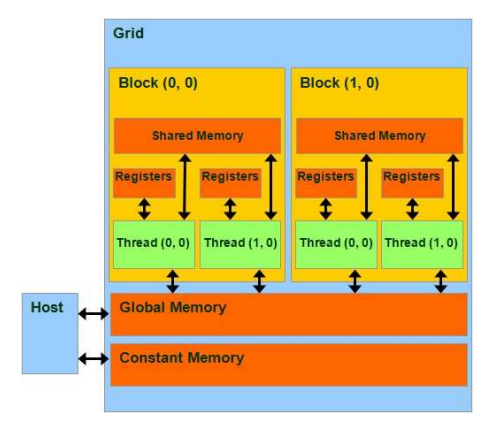
\includegraphics[scale=0.70]{images/cuda_memory.png}
	\label{fig:cudamemory}
\end{figure}

Global memory can be read and write in a kernel while constant memory can only be
read. However, access to the constant memory is much faster than the global memory because it can be cached. Shared memory is designed for the data communication for
threads in a block. This is fast but very limited. Each thread has several privates registers and is the fastest memory in GPU device. \marcio{Não entendi a frase seguinte??}\ed{It is used for the most frequently used in the program.} Since memory access contributes a lot in the computation time of the program, developers should take advantage of different kinds of memory. The key rule is that registers and share memory should be used as much as possible and the data that are not modified in the execution should be stored in the constant memory to have faster access.

\subsubsection{OpenCL}

After the release of CUDA, an alternative open standard general-purpose programming
API was released under the name OpenCL (Open Computing Language) ~\cite{Kirk:2012}.
Initially Developed by Apple and subsequently the Khronos Group, OpenCL allows
developers to harness the GPU and multi-core CPUs for general-purpose parallel
computation. However, unlike CUDA, OpenCL has multi-vendor and multiplatform
support thus allowing parallel code to be executed on AMD and NVIDIA GPUs
as well as x86 CPUs. This gives OpenCL the advantage of portability between
platforms. However, as Kirk and Hwu~\cite{Kirk:2012} noted, OpenCL programs can be inherently more complex if they choose to accommodate multiple platforms and vendors.
Developers must use different features from each platform to maximize performance
and so multiple execution paths dependent on the platform and vendor must be
included. This can result in each platform achieving a different execution time
depending on the input algorithm, mapping, and usage of platform-specific APIs
that may give an advantage to that specific platform. Kirk and Hwu also note
that the design of OpenCL is influenced heavily by that of CUDA and as a result
working with OpenCL can be very similar to CUDA. As with CUDA, regions of
the application that execute in parallel are encapsulated in kernels. OpenCL also
has a similar concept of CUDA blocks and threads which have been renamed to
Work group and Work item respectively. The current index of the block within the
grid of all blocks has also been renamed as the NDRange. To facilitate support for
multiple devices across platforms and vendors, OpenCL introduces the concept of
an OpenCL context. Each device is assigned to a context and work is scheduled
for execution in a queue for that context~\cite{Kirk:2012}. For additional information regarding OpenCL, we direct the reader to the Khronos Group OpenCL specification~\cite{opencl}.

\section{The AClang Compiler}
\label{sec:AClang}

Although OpenCL provides  a library that eases the  task of offloading
kernels  to  devices,  its  function  calls  are  complex,  have  many
parameters and  require the programmer  to have some knowledge  of the
device architecture's  features (e.g. block size,  memory model, etc.)
in order to enable a correct and effective usage of the device. Hence,
OpenCL  can  still  be  considered a  somehow  low-level  language  for
heterogeneous computing.

Introduced  through   OpenMP  4.0  the  new   \tit{OpenMP  Accelerator
	Model}~\cite{Liao2013}  proposes a  number of  new clauses  aimed at
speeding up the task  of programming heterogeneous architectures. This
model extends the concept of  offloading and enables the programmer to
use  dedicated directives  to  define offloading  target regions  that
control data movement between host  and devices.  Although most OpenMP
directives used  for multicore  hosts can also  be used  inside target
regions, the  new accelerator  model easies  the tasks  of identifying
data-parallel computation.

ACLang is an  open  source (\url{www.aclang.org})  LLVM/Clang
based compiler that implements the  OpenMP Accelerator Model.  It adds
an {\em  OpenCL runtime  library} to  LLVM/CLang that  supports OpenMP
offloading to  accelerator devices  like GPUs  and FGPAs.   The kernel
functions are extracted  from the OpenMP region and  are dispatched as
OpenCL~\cite{opencl}  or  SPIR~\cite{spir}  code   to  be  loaded  and
compiled by OpenCL  drivers, before being executed by  the device. This
whole  process is  transparent  and does  not  require any  programmer
intervention.

\begin{figure}[t]
	\caption{AClang compiler pipeline.}
	\centering
	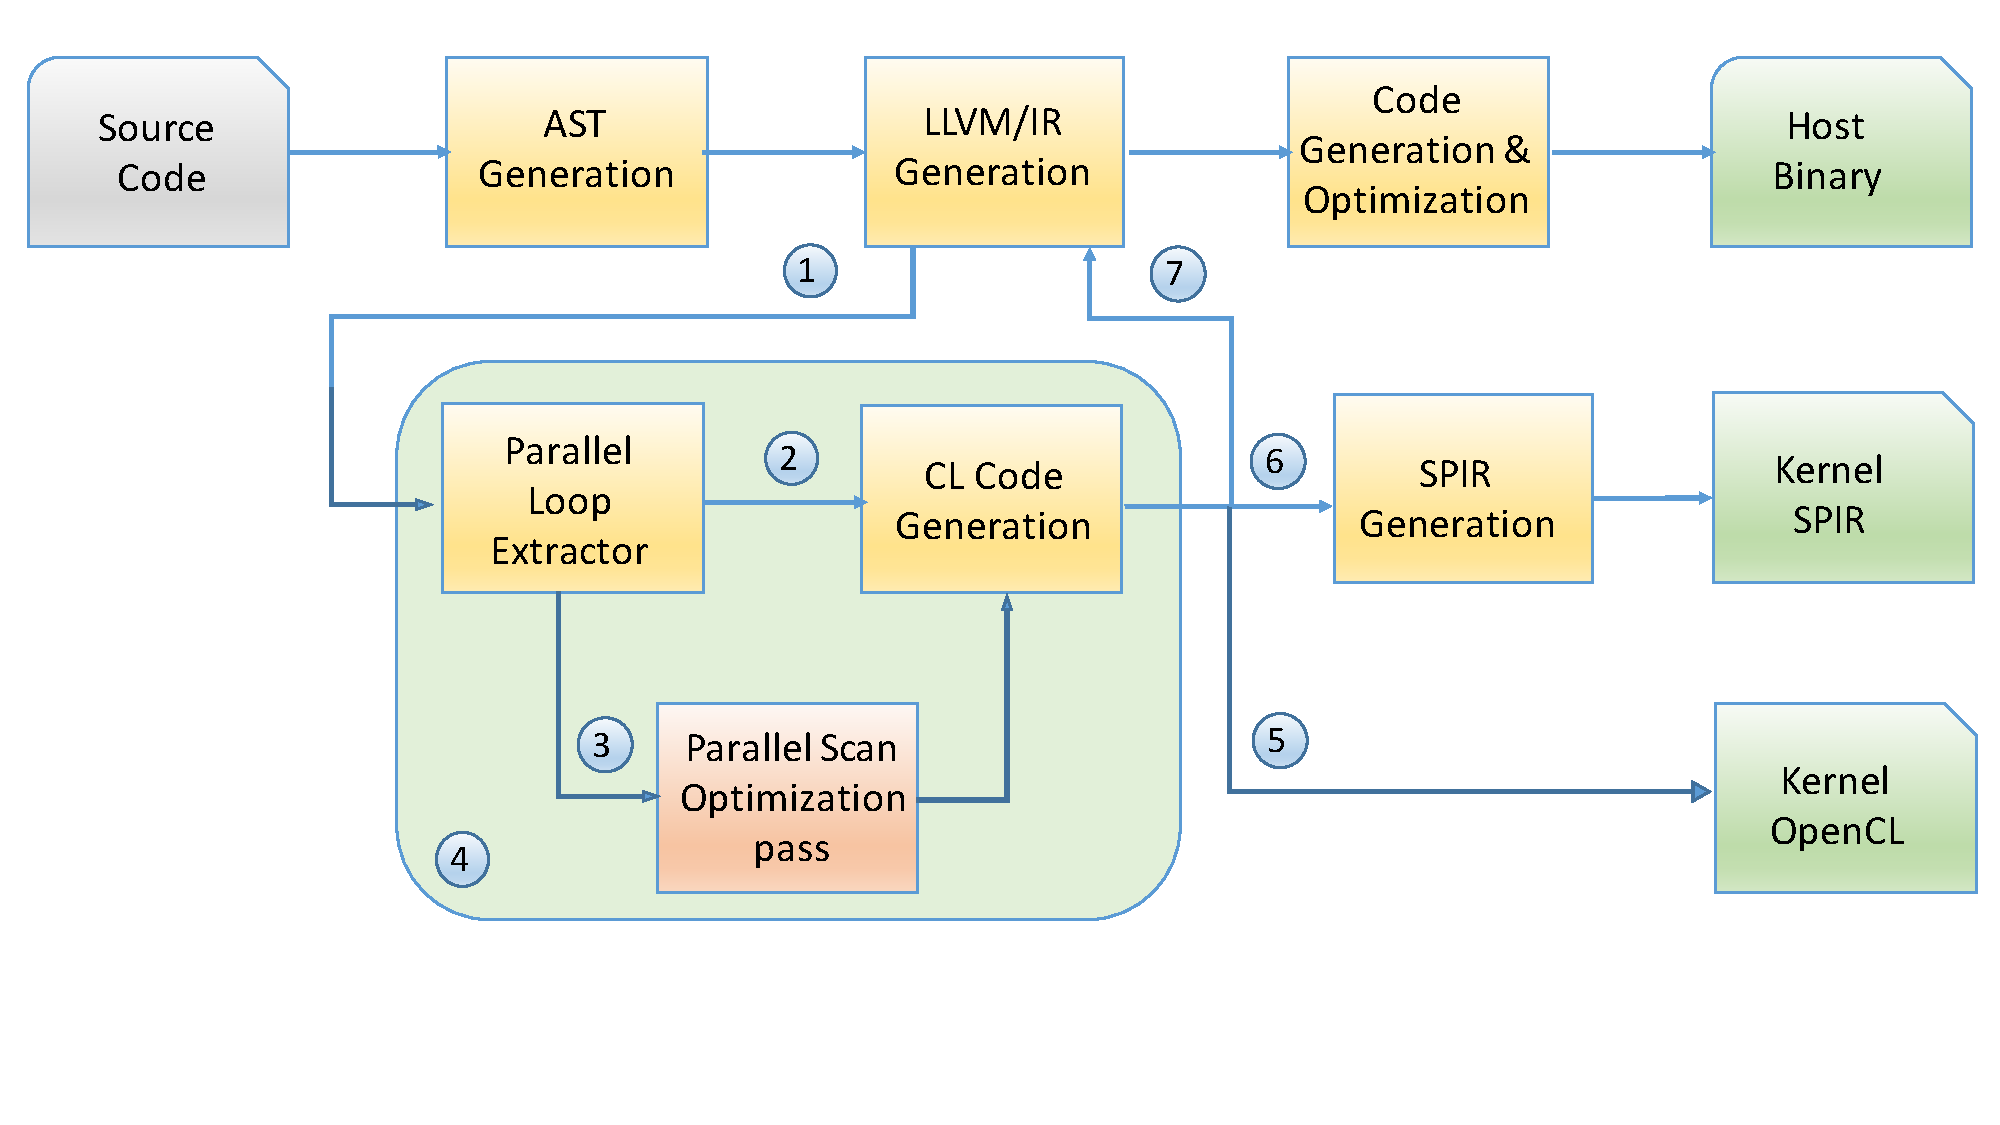
\includegraphics[scale=0.40]{images/aclang_scan.pdf}
	\label{fig:aclang}
\end{figure}


\rfig{aclang} shows  the AClang execution flow  pipeline with
emphasis on the \textit{Parallel Scan Optimization} pass.  The
LLVM IR generation phase handles the conversion of the AST
nodes  generated   by  the  Semantic  phase   into  LLVM  Intermediate
Representation\footnote{Historically,   this  was   referred  to   as
	\textit{codegen}}.  In this phase, the annotated loops are extracted
from     the      AST~\ding{182},     optimized~\ding{184},     and/or
transformed~\ding{183}  into  OpenCL  kernels in  source  code  format~\ding{186}
(see~\rsec{ScanInAClang}   for  more   details   on  the   Parallel Scan
optimization pass).   Kernels can also go  through the SPIR
generation pass~\ding{187} to produce kernel bit codes in SPIR format.
AClang's  transformation engine~\ding{185}  provides information
to  the LLVM  IR generation  phase~\ding{188} to  produce intermediate
code  that  calls  ACLang   runtime  library  functions.   These
functions are used  to perform data offloading and  kernel dispatch to
the  OpenCL  driver.

\chapter{The Parallel Scan}
\label{cap:Scan}

\section{The Scan algortihm}
\label{sec:ScanAlg}

In the 80's Hillis and Stelle~\cite{dataparallel} presented several algorithms
parallelized. To execute these algorithms, it was used on the Connection Machine System~\cite{themachine}. Thus, a very important observation of these algorithms
is that Hillis considered a unlimited number of processors, so they did not worry about that. The algorithms was tested with 65536 elements (maximum number of processors of The Connection Machine~\cite{themachine}).
One algorithm presented in the work mentioned aboves performs a sum of an array of numbers (see Figure \ref{fig:reductionhillis}). In this days this problem is known as $reduction$.\\
The main idea to solve the problems is to organize the addends at the leaves of a
binary tree and performing the sums at each level of the tree in parallel. Exist several ways to organize an array into a binary tree. Figure \ref{fig:reductionhillis} illustrates the method chosen by them. As an example, it is presented an array of 8 elements named $x_{0}$ through $x_{7}$. In this algorithm, for purposes of simplicity, the number of elements to be summed is assumed to be an integral power of two. There are as many processors as elements, and the line $4$ (in~\rlsts{HillisAlgorithms}{a}) causes all processors to execute the lines $5$ and $6$ (~\rlsts{HillisAlgorithms}{a}) in synchrony, but the variable k has a different value for each processor, namely, the index of that processor within the array. At the end of the process, $x_{n-1}$ contains the sum of the n elements.\\
As described in~\rlsts{HillisAlgorithms}{a} at each level
(iteration) $d$ of the tree, if the processor $k$ that meets the property of the line $5$
stored the sum of the neighbors at distance $2^{d-1}$ on his own position.
For  example, at  level $d  = 1$  of \rfig{reductionhillis} the processor $k = 1$ stored the sum of the neighbors at distance $2^{1-1} = 1$ (elements of $1$ and $0$) into the element at index $k = 1$, at the  next level of  the tree $d = 2$. The distance of the
neighbors will be $2^{2-1} = 2$ and so on until reach the last level where the root of the three holds the sum of all nodes in the array. The algorithm is computed in $O(log\ n)$ time, it performed $log\ n$ levels and each level is performed in parallel which means a constant time.

\begin{figure}[t]
	\centering
	\caption{Hillis and Steele reduction algorithm}
	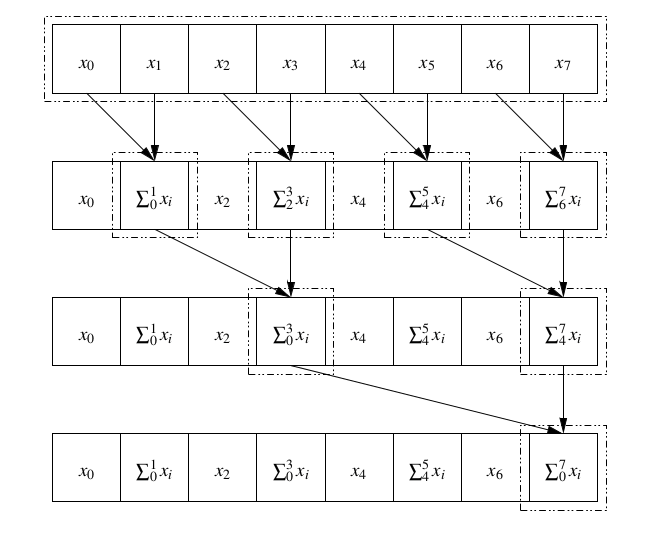
\includegraphics[scale=0.5]{images/reduction.png}
	\label{fig:reductionhillis}
\end{figure}

Another algorithm presented by Hillis and Steele~\cite{dataparallel} is the scan. They perceived that modifying only one line they can get all the partial sums of an array.
Looking at the simple summation algorithm explained above(\rlsts{HillisAlgorithms}{a}), it can be appreciated that most of the processors are idle most of the time. Line $5$ shows that during iteration $j$, only $n/2^{j}$ processors are active, and, indeed, half of the processors are never used. However, using the idle processors by allowing more processors to operate all the partial sums of the array can be computed from the previous algorithm explained with same amount of time that took to compute reduction $log\ n$. The key to understand this algorithm is to remember, in defining $\sum_{j}^{k}$ to mean $\sum_{i=j}^{k}x_{i}$, note that $\sum_{j}^{k}$ + $\sum_{k+1}^{m}$ = $\sum_{j}^{m}$. The algorithm replaces each $x_{k}$ by $\sum_{0}^{k}$: that is, the sum of all elements preceding and including $x_{k}$. In Figure \ref{fig:scanhillis}, this process is illustrated for an array of 8 elements.
The only difference between this algorithm and the earlier one is the test in the if statement in the partial-sums algorithm that determines whether a processor will perform the assignment (line $5$ to $14$). This algorithm keeps more processors active: During step $j$, $n - 2^{j}$ processors are in use; after step $j$, element number $k$ has become $\sum_{a}^{k}$ where $a = max(0, k - 2^{j} + 1)$. For  example, at  level $d  = 1$  of \rfig{scanhillis} the processor $k = 1$ stored the sum of the neighbors at distance $2^{1-1} = 1$ (elements of $1$ and $0$) into the element at index $k = 1$, the processor $k = 2$ stored the sum of the neighbors with the same distance $1$ (elements of $2$ and $1$) into the element at index $k = 2$ and son, at the  next level of  the tree $d = 2$. The distance of the neighbors will be $2^{2-1} = 2$ and the processor $k = 2$ stored the sum of the neighbors $2$ and $0$) into the element at index $k = 2$ (note that this element has the sum of $\sum_{0}^{0}$ to $\sum_{1}^{2}$ that is $\sum_{0}^{2}$) so on until reach the last level where all the nodes have the sum all its precedents elements, the element $k$ has the following sum $\sum_{0}^{k}$. The algorithm is computed in $O(log\ n)$ time, it has $log\ n$ levels and each level is performed in parallel which means a constant time.\\
In 1990, Guy  E. Blelloch~\cite{ScanAsPrimitive} proposed a new method to perform the scan parallel algorithm. For this new method is also used balanced trees. The idea is to build a balanced binary tree on the input data and sweep it from the leaves to the root to compute the all the partial sums. A binary tree with $n$ leaves has $d = log n$ levels, and each level $d$ has $2^{d}$ nodes. If it is performed one add per node, then we will perform $O(n)$ adds on a single traversal of the tree.

The key  idea in~\cite{ScanAsPrimitive} is  to build a  balanced binary
tree on the input data $x$ and  sweep it to and from the root, scanning
at each phase half  of the elements of the array.  The  tree is not an
actual  data structure,  but a  concept  used to  determine what  each
thread does at each one of the  two phases of the traversal.  The tree
representation is  shown in~\rfigs{upsweep}{downsweep} where  blue and
black arrows  represent read  operations of the  elements of  $x$ that
will be added, and orange arrows represent copy statements.

As  shown  in \rlstn{Parscan}{a}{b},  the  algorithm  consists of  two
phases:  \textit{up-sweep} and  \textit{down-sweep}.
In  the up-sweep phase,  described   in  ~\rlsts{Parscan}{a}  the  tree   is  traversed
bottom-up computing the scan of half of the internal nodes of the tree
in~\rfig{upsweep}.  As described in~\rlsts{Parscan}{a} at each level
(iteration)  $d$  of   the  tree  neighbors  at   distance  $2^d$  are
accumulated       into        the       elements        at       index
$k + 2^{(d+1)} - 1, k = 0 \ldots \lceil n/2 \rceil$ of the array (line
18). For  example, at  level $d  = 0$  of \rfig{upsweep}  neighbors at
distance $2^{(0+1)}  - 1  = 1$  are accumulated  into the  elements at
index $k  + 1$, at the  next level of  the tree.  The distance  of the
neighbors  that  are   accumulated  doubles  as  the   tree  level  is
incremented  (e.g.  the  distance is  2 at  level $d  = 1$)  until the
partial sum  at $x[i-1]$  is computed.   This phase  is also  known as
\textit{parallel reduction},  because after this phase,  the root node
(the last node in the array) holds the sum of all nodes in the array.\\
In  the down-sweep  phase,  the  tree is  traversed  top-down and  the
partial sums computed in the previous phase are propagated downward to
accumulate  with the  entries which  did not  have their  partial sums
computed  previously  in the  up-sweep  phase.   The phase  starts  by
inserting zero at the  root of the tree. Then at  each step, each node
at the current tree level will: (i)  sum its value to the former value
of its left child and store the  result into its right child; and (ii)
copy its own value to its  left child.  For example, consider the node
at index $7$  level $d = 1$  of the tree in  \rfig{upsweep}. That node
has two children, a left child at index $5$ and a right child at index
$7$.  Hence,  during the down-sweep  phase two operations  will occur:
(i) the value at  index $7$ is summed to the value  at index $5$ (left
child of index  $7$) and is stored  into the right child  of index $7$
(index $7$ itself); and (ii) the value at index $7$ is copied to index
$5$ to be used  in the next level $d = 0$ (orange  arrow to left child
of index $7$). The algorithm  performs $\mathcal{O}(n)$ operations in the first
phase (\textit{up-sweep}) and for every level of this phase ($log\ n $ levels) is computed in $\mathcal{O}(1)$ (because is done in parallel) hence the total time is computed in $\mathcal{O}(log\ n)$, similarly for the second phase (\textit{down-sweep}) the total of operations is $\mathcal{O}(n)$ between adds ($n-1$) and swaps ($n-1$) moreover the computed time is $\mathcal{O}(log\ n)$. So the total number of operation of parallel scan is $\mathcal{O}(n)$ and computed time is $\mathcal{O}(log\ n)$ time.\\
 

\begin{figure}[t]
	\lstset{basicstyle=\scriptsize}
	\begin{lstlisting}[label=lst:HillisAlgorithms, caption={The parallel scan and reduction implementation proposed Hillis and Steele}, escapeinside={(*}{*)}]
	(a) Parallel Reduction

		for(int d = 1; d <= log2(n); d++)
			for(int k = 0 ; k < n ; k++){ //In parallel
				if( (k+1)%2^d == 0 ){
					x[k] = x[k - 2^(d-1)] + x[k];
				}
			}

	(b) Parallel Scan

		for(int d = 1; d <= log2(n); d++)
			for(int k = 0 ; k < n ; k++){ //In parallel
				if( k >= 2^d ){
					x[k] = x[k - 2^(d-1)] + x[k];
				}
		}

	\end{lstlisting}
\end{figure}

\begin{figure}[t]
	\centering
	\caption{Hillis and  Steele scan algorithm}
	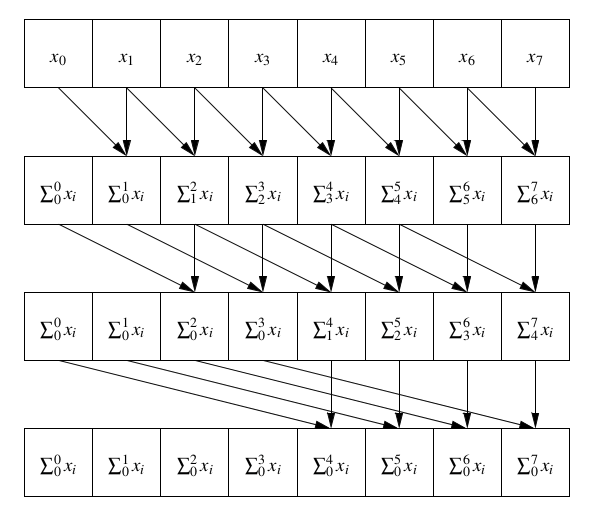
\includegraphics[scale=0.5]{images/hillisscan.png}
	\label{fig:scanhillis}

\end{figure}

In 2005, Horn~\cite{GPUGems2} proposed a first version of scan parallel for GPUs, this proposal was based in~\cite{dataparallel}, this implementation is more realist and limited. As was mentioned before for the work of~\cite{dataparallel}, they did not worry about the number of processor. They considered that it is possible to have a number of processors equal to the size of the input (not real situation in these days).
So the proposed of Horn was limited by the block size of the GPU device, in our days this size could be until 2048. Horn proposed the method using it at solution of the problem $Stream Compaction$. That problems is defined as follow: given an input vector, and one key value. It is necessary to reorder the input that the elements that have the same value of the key are moved towards to the end of the vector. The rest of the elements are moved towards to the begin keeping the original order between them (See Figure~\ref{fig:desire}). Remember that for this version of scan, the complexity is $log n$ and order of the operation is in order of $n log\ n$.\\

In 2007 Mark Harris et al.~\cite{harris2007parallel} proposed a new implementation of scan parallel algorithm, this version is based in the work of Blelloch~\cite{ScanAsPrimitive}. In the last method explained, proposed by Horn the number of operations is in order of $O(n log\ n)$ meanwhile the simple serial version of scan performs in order of $O(n)$ operations as well as Blelloch's version. That was one of Harris's main motivations, the possibility of at least achieve the same order of operations than the serial version. So, he implemented a method to solve the scan operation base in the work of Blelloch for a GPU. However, that implementation was the same problem of Horn's implementation, the algorithm only works for an small arrays, because is limited by a thread block. Thereby, the main contribution of Mark Harris was to design of an algorithm to be able to be use it for large arrays.
The basic idea is simple. It is divided the large array into blocks, each of them can be scanned by a single thread block, and then it is computed the scan operations for the blocks and write the total sum of each block to another array of block sums. Then scan the block sums, generating an array of block increments that that are added to all elements in their respective blocks. For example (see Figure~\ref{fig:largescan}), let $N$ be the number of elements in the input array, and $B$ be the number of elements processed in a block. It is allocated $N/B$ thread blocks of $B/2$ threads each. (Here it is assumed that N is a multiple of $B$. A choice is according of GPU Series. It is used the scan algorithm of the previous sections to scan each block $i$ independently, storing the resulting scans to sequential locations of the output array~\ding{172}. It was made one minor modification to the scan algorithm. Before zeroing the last element of block $i$ (the block of code labeled $B$ in line $15$ in~\rlst{Parscan}), It is stored the value (the total sum of block $i$) to an auxiliary array represented by $\sum$~\ding{173}. Then scan $\sum$ in the same manner, writing the result to an array represented by $\sigma$~\ding{174}. Then add $\sigma[i]$ to all elements of block $i$~\ding{175}. After making all the previous steps, it is obtained the final array of scanned values. 

\begin{figure}[t]
	\centering
	\caption{Example of scan application}
	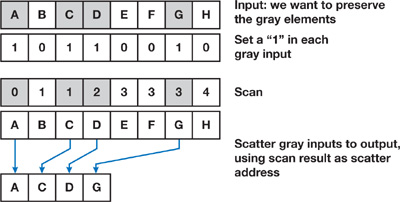
\includegraphics[scale=1.0]{images/desireElements.jpg}
	\label{fig:desire}
\end{figure}

\begin{figure}[t]
	\centering
	\caption{Parallel scan in $\mathcal{O}(log\  n)$}
	\subfloat[Up-sweep phase]{
		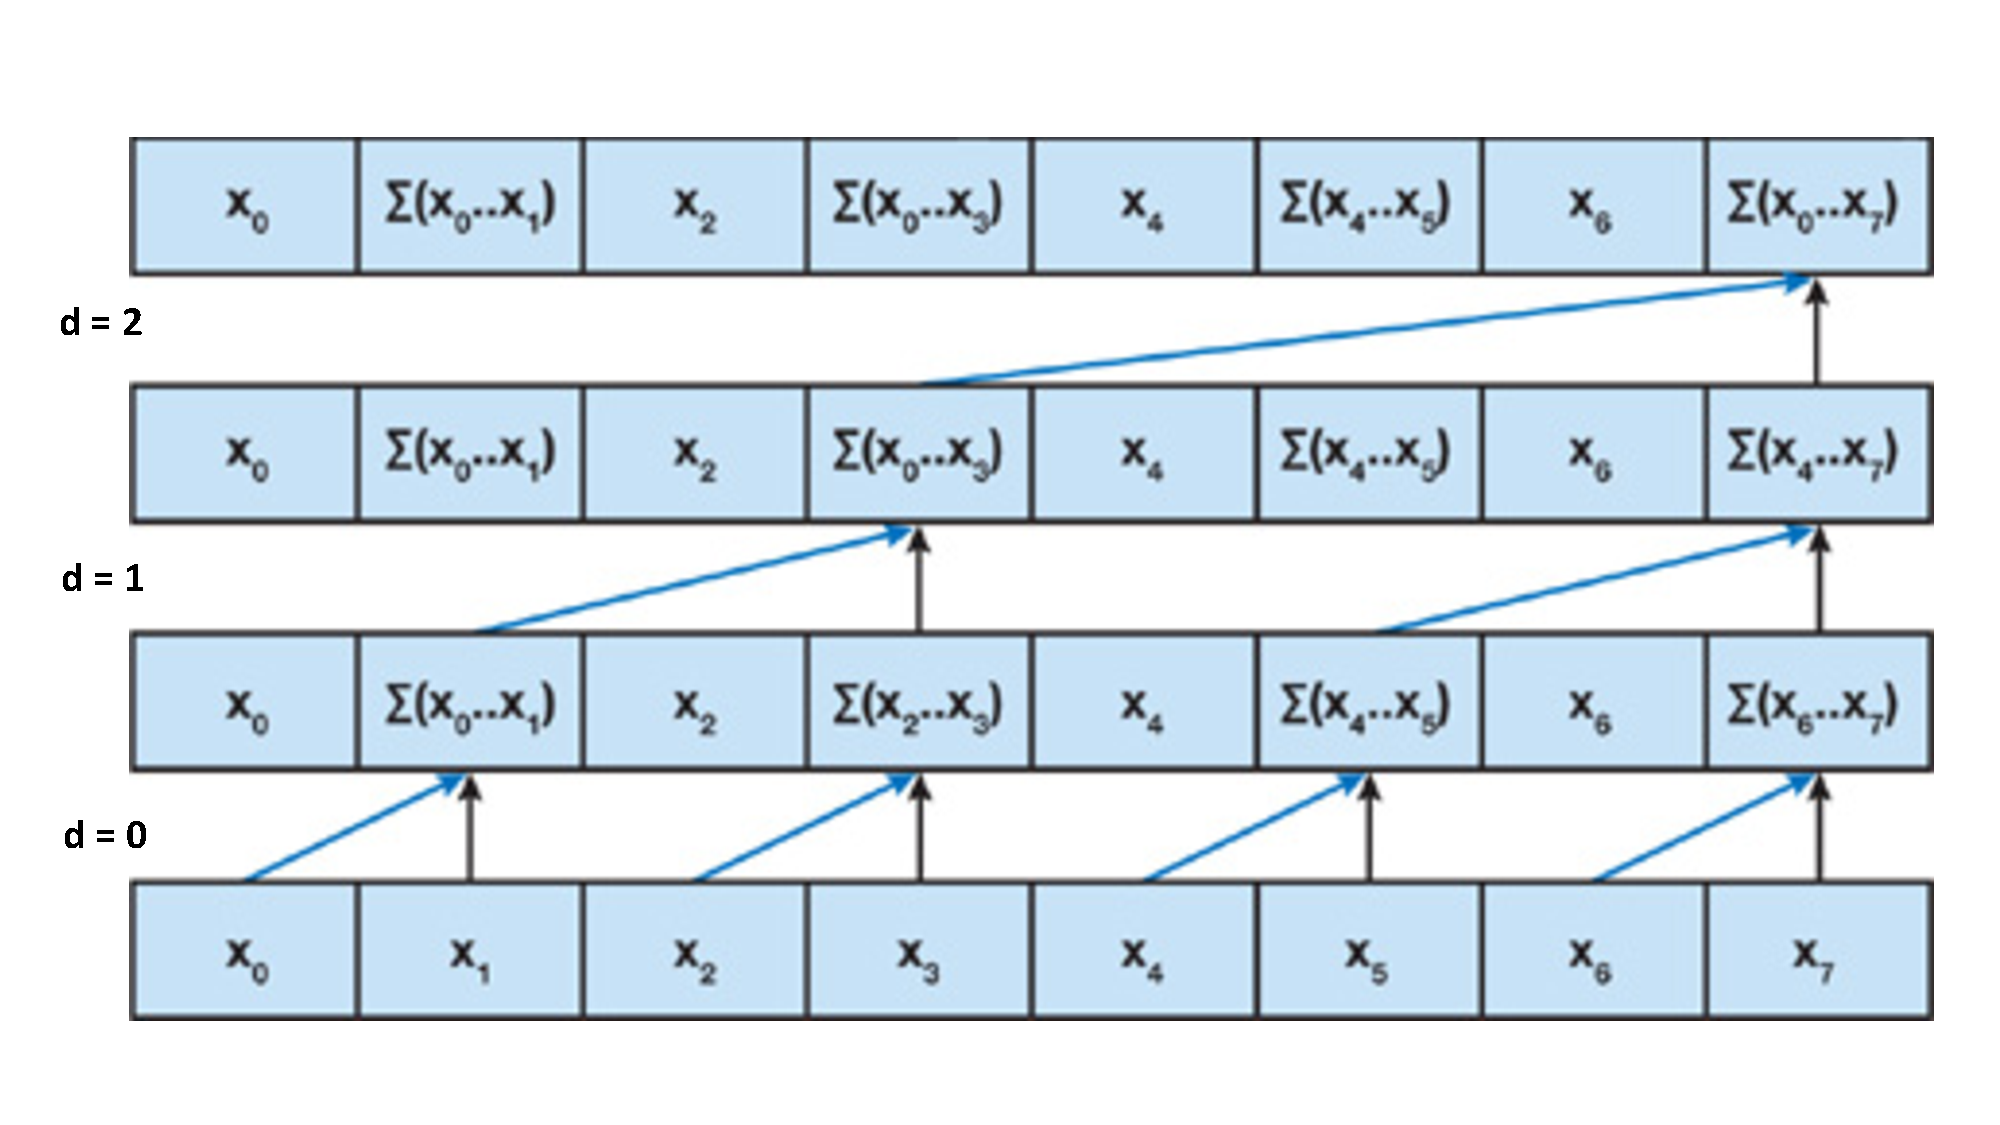
\includegraphics[scale=0.35]{images/upsweep.pdf} \label{fig:upsweep}
	}
	\vfill
	\subfloat[Down-sweep phase]{
		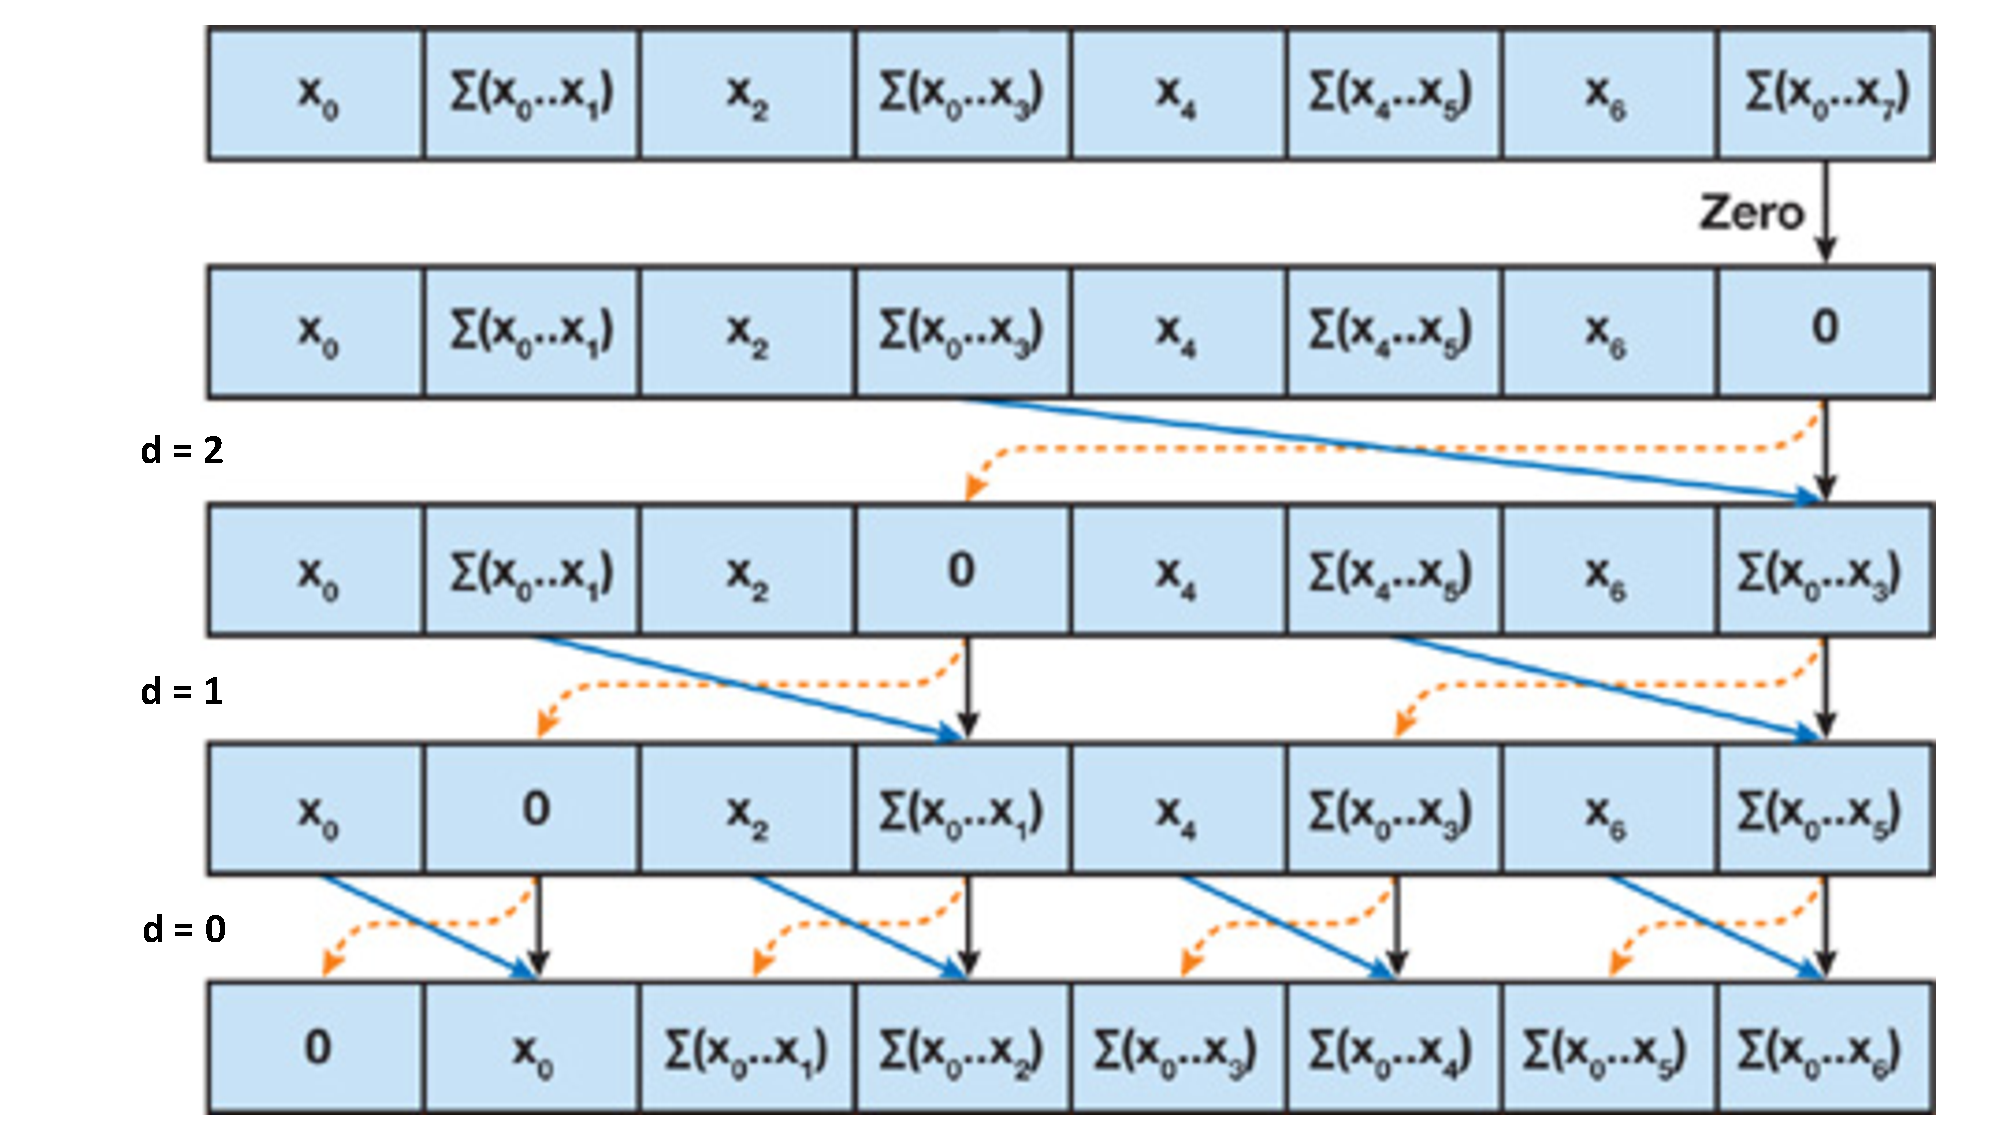
\includegraphics[scale=0.35]{images/downsweep.pdf}\label{fig:downsweep}
	}
\end{figure}
.
\begin{figure}[t]
	\lstset{basicstyle=\scriptsize}
	\begin{lstlisting}[label=lst:Parscan, caption={The parallel scan implementation proposed by Blelloch}, escapeinside={(*}{*)}]

	(a) Up-sweep phase of scan parallel implementation

	x[0] = 0;
	for(d = n >> 1; d > 0; d >>= 1){
		// We parallelize this section
		for(k = 0 ; k < n ; k += (1<<(d+1)) ){
			x[k + (1<<(d+1)) - 1] = x[k + (1<<d) -1] +
			x[k + (1<<(d+1)) - 1];
		}
	}

	(b) Down-sweep phase of scan parallel implementation

	x[n-1] = 0;
	for(d = log2(n); d >= 0 ; d--){
		// We parallelize this section
		for(k = 0 ; k < n ; k += (1<<(d+1))){
			t = x[k + (1<<d) - 1];
			x[k + (1<<d) - 1] = x[k + (1<<(d+1)) - 1];
			x[k + (1<<(d+1)) - 1] = t + x[k + (1<<(d+1)) - 1];
		}
	}
	\end{lstlisting}
\end{figure}

\begin{figure}[t]
	\centering
	\caption{Scan for large arrays by Mark Harris et al.}
	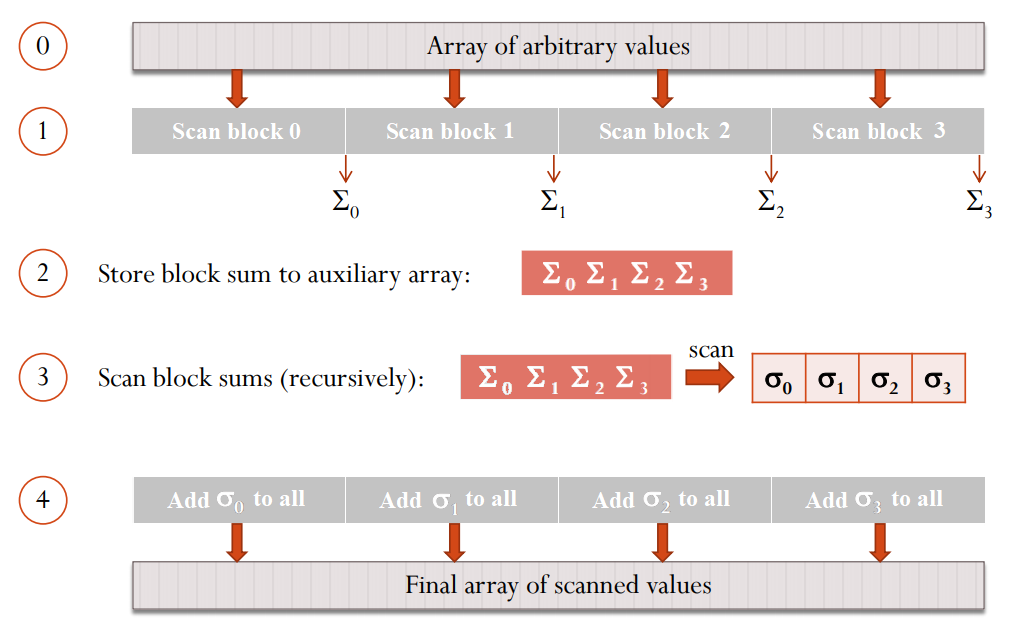
\includegraphics[scale=0.4]{images/largescan.png}
	\label{fig:largescan}
\end{figure}

\begin{figure}[t]
	\lstset{basicstyle=\scriptsize}
	\begin{lstlisting}[label=lst:ClangScan, caption={Pseudocode of Scan Parallel implementation in Aclang}, escapeinside={}]
	(a) Get information from omp scan clause

	I = S.clauses().begin(), E = S.clauses().end();
	OpenMPClauseKind ckind = ((*I)->getClauseKind());
	if (ckind == OMPC_scan){ //Checking if the clause extracted is our Scan clause.
	 OMPVarListClause<OMPScanClause> *list = cast<OMPVarListClause>cast<OMPScanClause>(*I);
	}

	(b) Detecting programmer needs
	 if (num_mapped_data == 1) {
		 ...
	 }
	else {
	if (num_mapped_data > 2) {
	 llvm_unreachable("Unsupported scan clause with more than two mapped data");
	}
	if (MapClauseTypeValues[0] == OMP_TGT_MAPTYPE_TO ||
	    MapClauseTypeValues[0] == OMP_TGT_MAPTYPE_TOFROM) {
		...
	}

	(c) Preparing the scan algorithm parameters and openCL environment

	ThreadBytes = EmitRuntimeCall(CGM.getMPtoGPURuntime().cl_get_threads_blocks(), KArg);
	Q = dyn_cast<ArrayType>(Q.getTypePtr())->getElementType();
	OpenMPScanClauseOperator op = cast<OMPScanClause>(*I)->getOperator();

	EmitRuntimeCall(CGM.getMPtoGPURuntime().cl_create_read_write(), Size);
	EmitRuntimeCall(CGM.getMPtoGPURuntime().cl_create_program(), FileStrScan);

	EmitRuntimeCall(CGM.getMPtoGPURuntime().cl_create_kernel(), FunctionKernel_0);
	EmitRuntimeCall(CGM.getMPtoGPURuntime().cl_create_kernel(), FunctionKernel_1);
	EmitRuntimeCall(CGM.getMPtoGPURuntime().cl_create_kernel(), FunctionKernel_2);
	EmitRuntimeCall(CGM.getMPtoGPURuntime().cl_release_buffer(), Aux);

	(d) Customing the scan generator

	 CLOS << "#pragma OPENCL EXTENSION cl_khr_fp64 : enable\n\n";
	 std::string includeContents = CGM.OpenMPSupport.getIncludeStr();
	 if (includeContents != "") {
		 CLOS << includeContents;
	 }
	 switch (op) {
		 case OMPC_SCAN_add:
		 case OMPC_SCAN_sub:
			 initializer = "0";
		...
	 }
	 if (initializer == "") {
	 } else {
		 CLOS << "\n#define _initializer " << initializer;
	 }

	CLOS << "\n#define _dataType_ " << scanVarType.substr(0, scanVarType.find_last_of(' ')) << "\n";
	CLOS.close();


	\end{lstlisting}
\end{figure}

\begin{figure}[t]
	\lstset{basicstyle=\scriptsize}
	\begin{lstlisting}[label=lst:TemplateScan, caption={Template to generate the final kernel of scan parallel algorithm}, escapeinside={}]
	(a) Header for every kernel
	Header_kernel = """
		__kernel void kernel_0 (__global _dataType_ *input,
		__global _dataType_ *S,
		const int n) {
	"""

	(b) Kind of Operation

		Oper_0_basic = """	block[bi] = block[bi] _operation_ block[ai];  """
		Oper_0_user  = """	block[bi] = _operation_(block[bi], block[ai]);"""


	(c) Vector result

		Tail_input_basic  = """	input[gid]  = input[gid] _operation_ S[bid];  """
		Tail_output_basic = """ output[gid] = input[gid] _operation_ S[bid]; """

	\end{lstlisting}
\end{figure}


\section{Scan clause implementation in AClang}
\label{sec:ScanInAClang}

\begin{figure}[t]
	\centering
	\caption{Algorithm to perform a block sum scan}
	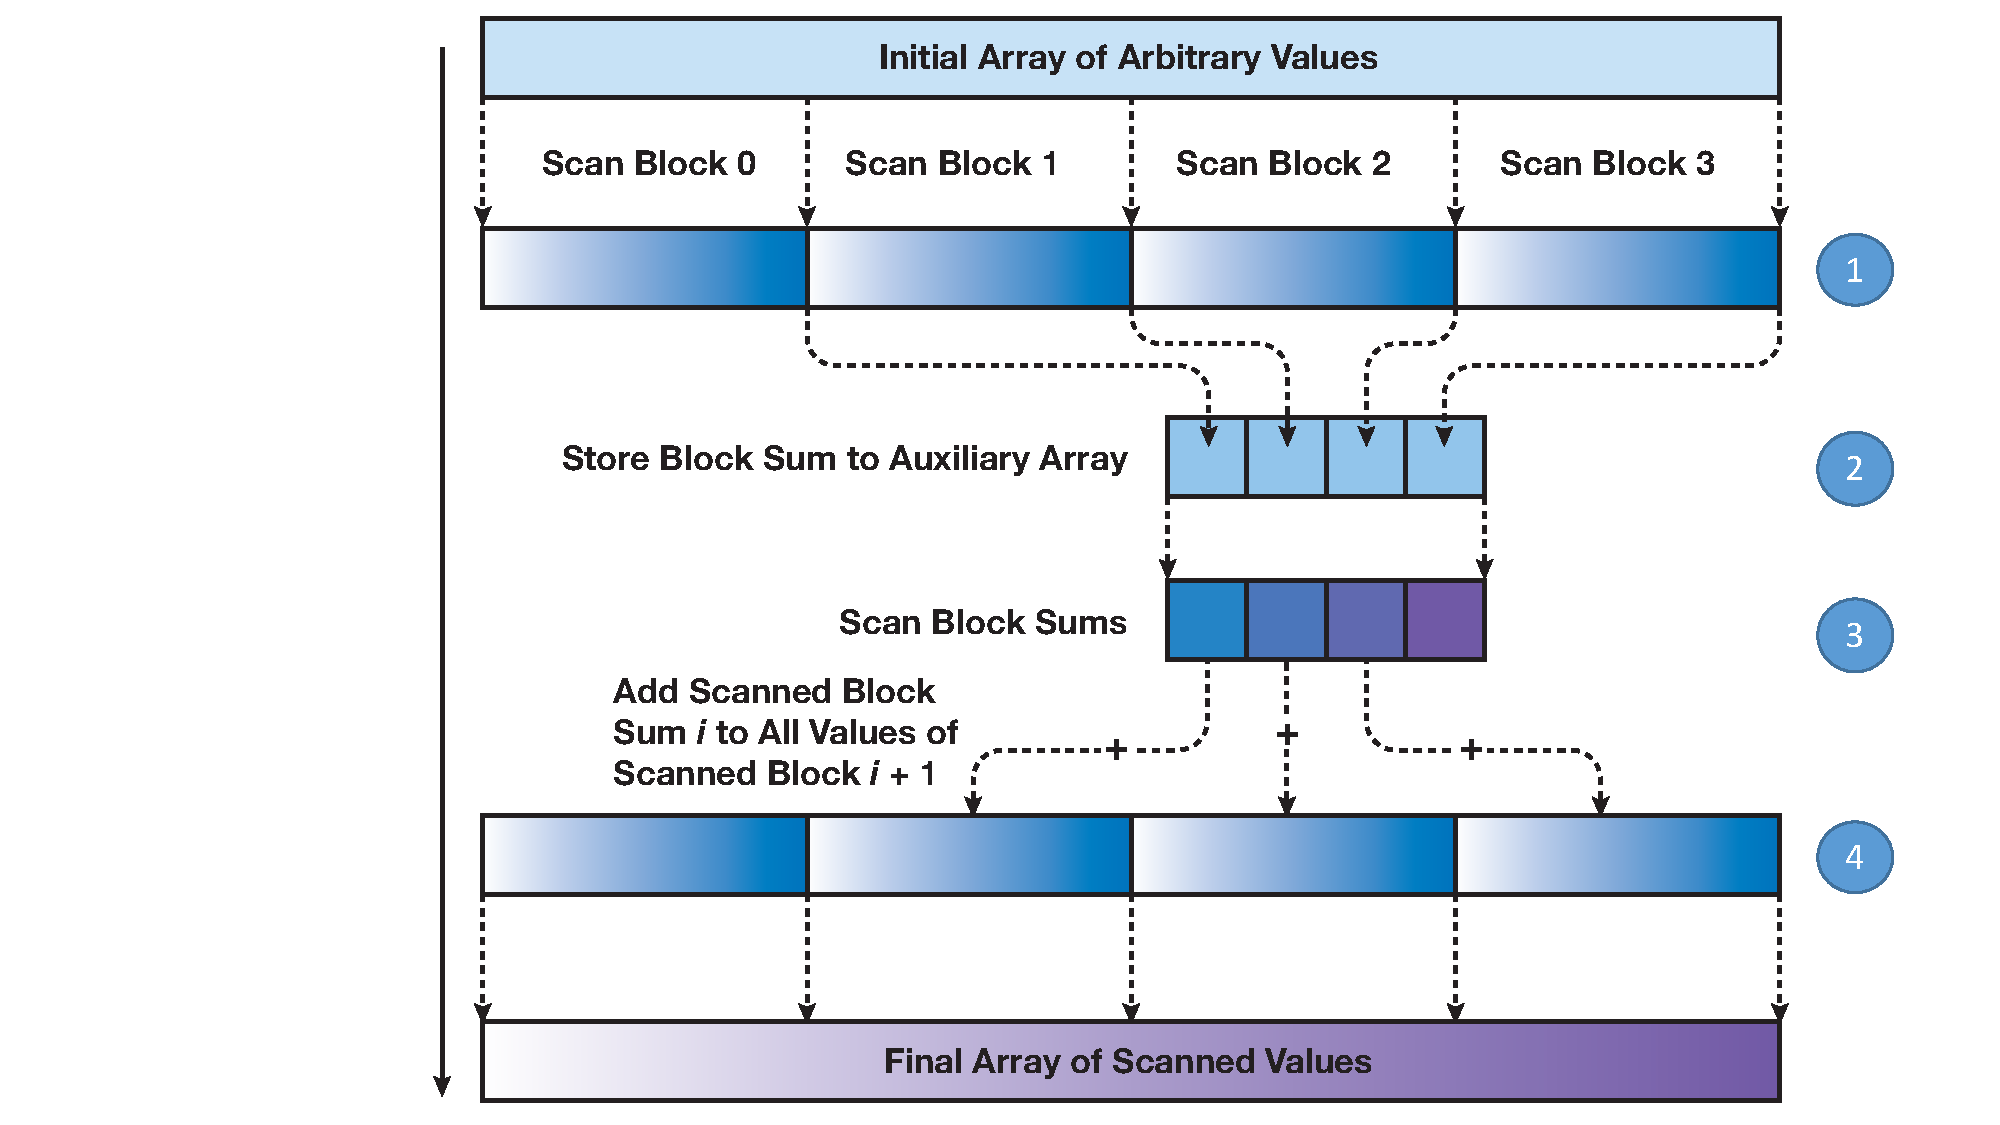
\includegraphics[scale=0.45]{images/phaseScan.pdf}
	\label{fig:scheme}
\end{figure}


The Parallel Scan Optimization  pass~\ding{184} shown in \rfig{aclang}
is responsible  for implementing the scan  clause. This implementation
is    based   on    the   best    parallel   scan    algorithm   known
today~\cite{Sengupta:2007}       and       is       detailed       in
\rsec{ScanAlg}.  Nevertheless, the  effectiveness  of  that algorithm  is
increased  when it  runs within  a thread  block within  which it  can
leverage on data locality.

In order to apply the  parallelized scan from~\rsec{ScanAlg} to data sets
larger than  a single thread block,  an extended four step  method was
proposed~\cite{harris2007parallel}. This method applies twice the  scan
algorithm described in \rlstn{Parscan}{a}{b} to spread the scan of each
block to all blocks  of the array.  Such method is  shown in the block
diagram of \rfig{scheme} where each  number corresponds to one step of
the method.   In the first  step, the  method divides the  large input
array  into  blocks  that  are   scanned  each  by  a  single  thread
block~\ding{182} using  the algorithm  from ~\rsec{ScanAlg}.   During the
second step,  the total sum  of all elements  of each block  (i.e. the
value in the  last element of the scanned block)  is transfered to the
corresponding entry of  an auxiliary array ~\ding{183}.   In the third
step, using again  the algorithm in~\rsec{ScanAlg}, the  method scans the
auxiliary  array, and  writes the  output  at another  array of  block
sums~\ding{184}.  At  the end  of this  third step  each entry  of the
array of block  sums contains the partial sums of  all elements of the
blocks up to that entry (inclusive).   Finally in the fourth step,
for each block the method adds the previous block sums  to the elements of the current
block~\ding{185}.

The following paragraph describes how ACLang implements the parallel scanning algorithm. This process makes the necessary calls to the AClang runtime library and populates a template that will execute the scan algorithm with the program data (e.g., type of data to be carried out the scan, the scan operation, the output vector).

\begin{figure}[t]
	\lstset{basicstyle=\scriptsize}
	\begin{lstlisting}[label=lst:ScanKind, caption={Pseudocode of Scan Parallel implementation in Aclang}, escapeinside={}]
	(a) Standard way to write scan algortihm
		y[0] = 0;
		for(i = 1 ; i < n ; i++)
			y[i] = y[i-1] + x[i-1];


	(b) Alternative way saving memory to write scan algorithm
		int aux1 = x[0], aux2;
		x[0] = 0;
		for(i = 0 ; i < n ; i++){
			aux2 = x[i];
			x[i] = x[i-1] + aux;
			aux = aux2;
		}

	\end{lstlisting}
\end{figure}

In the first step, the algorithm obtains the pieces of information of the
omp scan clause, as detailed in \rlst{ClangScan}{a}, lines 3 through
20.

Lines 3 to 7 get the list of variables and the kind of operation
  associated with the scan clause.

In \rlst{ClangScan}{b}, it's recovered the buffer where the result of the scan
algorithm will be written, as can be seen in \rlstn{ScanKind}{a}{b}.
In \rlstn{ScanKind}{a} is a standard way to write scan algorithm (input and output vectors). In \rlstn{ScanKind}{b} is showed a second way to write scan algorithm,
in this case it's necessary just an input data and auxiliary variables.

Lines 24 to 34 retrieve the
scan parameters and and makes an initial configuration of OpenCL. Line $24$ computes the number of threads per block and the
number of blocks. That will be used to call the sub-routines of the parallel scan algorithm. This is a very important step because as mentioned before, the algorithm only works for input sizes that are powers of 2 ($2^{k}$). So when the
size is not a power of two, It's impossible to solve the problem. Hereby, to fix
it, it's founded the closest higher number that is a product of two powers of
two. Let's represent the number of blocks as $B$ and the number of threads per
block as $T$.\\ For example, if the size of the input data is $12$, the closest number with the properties mentioned before is $16$, where we found more of one solution
such as ($B$:1 - $T$:16), ($B$:2 - $T$:8), ($B$:4 - $T$:4) and so on.
Attention, in some cases it's possible to find some solution with $T$ bigger
than the threads provides for the architecture used. Thus, $T$ is limited
according of the architecture programmer features, similarly for $B$.\\
Therefore, the maximum size to compute the scan algorithm is limited for the
resources provided in the architecture, later in \ref{cap:Conclusion} it will
show a proposal to extend that limit.
Line 25 retrieves the type of variable in which the
program is performing the scan operation. This variable can be of type int,
double, float, but can also be a new user-defined type. In this case, it is
mandatory for this new type to be defined within the "omp declare target"
clauses (see example in \rlst{pol}).

Line $26$ find the operator that the programmer defined to use in the scan
algorithm. Attention, this operator should be a binary associative operator to
could use the scan algorithm, the most common are: ($+$, $*$, $\&$, $||$,
$max$, $min$). In the case that a new variable was defined it is mandatory
define an operator for this variable (See example in \rlst{pol}).

Line $28$ does a needed step to execute the scan algorithm, it
created an auxiliary buffer (as can see in \ref{fig:scheme} ~\ding{183}).
Aclang provides a series of methods in the {\it CodeGenModule} class for
calling the runtime library responsible for interfacing with the OpenCL
drivers. Those functions have the following structure:
$CGM.operation1.MPtoGPURuntime().operation2$.  Lines $29$ to $33$ generate code
for the runtime library to call the OpenCL driver to compile the kernels and
dispatch then for execution.

Lines $31$ to $33$ execute the necessaries kernels to compute the scan
algorithm. Line $31$ computes the scan for every single block thread
independently (as can see in \ref{fig:scheme} ~\ding{182}). Line $32$ executes
the second kernel that is in charge to computed the sum of accumulates from the
auxiliary vector (as seen in \ref{fig:scheme} ~\ding{184}). Line $33$ executes
the kernel in charge to distributes the corresponding accumulates to the
positions on the result vector (as can see in \ref{fig:scheme} ~\ding{185}).

Finally, line $34$ transfers the solution vector data to the programmer desired
vector, as we mentioned before, the programmer has two options to receive the
result vector.

\subsection{The Template}
\label{sec:template}

This section aims to explain how it is built the code of the parallel scan
algorithm.  Remember that the algorithm is based on the best algorithm known
today~\cite{Sengupta:2007}.

To summarize this section, it can be said that the algorithm has only three
parameters, those parameters could be different according to the applications.
The first one is the  type of variable, the second one is the operator defined
for the variable used. Finally the third one refers to the need of the
programmer, exactly refers to the use of new types of variables and operators.
Additionally, the programmer has two options to recover the result vector.
Thereby, as was mentioned before, all the information is recovered in the
compilation phase to be used to generate the kernel to execute the parallel
scan algorithm.

\rlst{TemplateScan}{a} defineds the header for each kernel. This example shows
the header of the first kernel. It can be appreciated that it is necessary to
define the variable $dataType$. As was mentioned before, that information was
extracted from the clause scan. As expected, every kernel that involves the use
of the variable type, it was replaced $dataType$ for the real variable type.

\rlst{TemplateScan}{b} defineds how the program will perform the calculations
between two variables. It refers to use a new operation defined for a new
variable type. Is possible to operate two variable in a simple way for a
primitive variables, for example for two variables $x$ and $y$ of type $int$ we
will use the line $10$ to compute the result.

On other hand, when the programmer defined a new type of variable, he must
define also its binary associative operator to be able to use the scan
algorithm. In this case, the operation can't be computed in a simple way, the
operation has to be defined in the section "omp declare target" for the
programmer. That information is recovered from the scan clause as a function
and the way to use this new operation was specified in the line $11$.

Finally, the last component of the template \rlst{TemplateScan}{c} refers to
where the programmer wants to save the result vector. Line $16$ represents when
the programmer needs a new vector to save the result. Line $17$ refers to the
programmer wants to save the result vector in input data vector.

Back to \rlst{ClangScan}{d}, Line $38$ fillings a standard header. Lines $39$
to $42$ analyze if the programmer defined a new type of variable with its
respective operator. If is true, that information is placed immediately after
the header mentioned before.

Lines $43$ to $52$ define the neutral value according to the operation, a
neutral value is defined by the operation ($a$ = $a$ $\oplus$ $neutralValue$)
where $a$ is any variable $\oplus$ is an operator, as we can see, when we
operate any variable with the neutral. For example, for the sum operation, the
neutral value is $0$, for the multiplication is $1$ and so on. This information
is necessary because the scan algorithm needs it. When it is worked with a
basic operation, for default this neutral is defined internally, however when
the programmer defined a new type of variable, it is mandatory define the
neutral value in the section "omp declare target"

Line $54$ defines the word $dataType$, it represents the type of variable that
is used for the programmer. Finally, line $55$ closes the file that will
perform the scan parallel algorithm. Remember, the explained is a very
summarized code of the total process. The aims to explain that code is to show
the mainly components to understand the process to how pass from the omp clause
to OpenCL code. Many informations have been left aside for reasons of priority.
To see a final version of the template for one example, see \rcap{ScanUse}.

\chapter{Using Scan}
\label{cap:ScanUse}

\section{Radix Sort}
\label{sec:Quicksort}

A sorting algorithm puts elements of a list in certain order. This section
presents Radix Sort algorithm parallelized through of scan operator. It is
well know how Radix Sort algorithm works.  For this reason, the section
focused on explaining the parallelized version.

The basic idea is to considerer each element to be sorted digit by digit, from
least to most significant. For every digit the elements will be rearranged.
Let’s take a simple example of 4 elements with 4 binary digits in its
representation. \rlst{radexample} shows a visual representation of how the
algorithm works.

\begin{figure}[t]
	\lstset{basicstyle=\scriptsize}
	\begin{lstlisting}[label=lst:radexample, caption={Radix Sort
	algorithm basic idea}, escapeinside={(*}{*)}]
	1) Elements representation
	Element #    1       2       3       4
	Value:       7       14      4       1
	Binary:      0111    1110    0100    0001

	2) At first step, Radix sort algorithm rearranges the elements by the values of
	   the bit analized(bit 0):
	Element #    2       3       1       4
	Value:       14      4       7       1
	Binary:      1110    0100    0111    0001
	bit 0:       0       0       1       1

	3) Finalized the first step, it is neccesary analize the next bit (bit 1):
	Element #    3       4       2       1
	Value:       4       1       14      7
	Binary:      0100    0001    1110    0111
	bit 1:       0       0       1       1

	4) And so on (bit 2):
	Element #    4       3       2       1
	Value:       1       4       14      7
	Binary:      0001    0100    1110    0111
	bit 2:       0       1       1       1

	5) And move them again:
	Element #    4       3       1       2
	Value:       1       4       7       14
	Binary:      0001    0100    0111    1110
	bit 3:       0       0       0       1

	\end{lstlisting}
\end{figure}

\marcio{Maicol: Os itens abaixo precisam ser reescritos. Não está claro a explicação do algoritmo}
But, How can \rlst{radexample} do parallel?
The next steps show how to do it.
\begin{enumerate}
\item Generate a vector of the list (bit in common, starting form the least significant bit)
where every bit that is 0 in the new vector is 1 else the value is 0.
\item Scan the vector, and record the sum of the predicate in the process. Notice, Scan
algorithm works for arrays of arbitrary size instead of $2^{n}$ size, however as how was
explained before the propose resolves for any arbitrary size.
\item Flips bits of the predicate, and scan that.
\item Move the values in the vector with the following rule:
\begin{enumerate}
\item For the $i^{th}$ element in the vector:
\item If the $i^{th}$ predicate (vector generate in the step 1) is TRUE, move the $i^{th}$
value to the index in the $i^{th}$ element of the predicate scan.
\item Else, move the $i^{th}$ value to the index in the $i^{th}$ element of the opposite array
of the Predicate Scan plus the sum of the original Predicate.
\end{enumerate}
\item Move to next significant bit (NSB).
\end{enumerate}


\begin{figure}[t]
	\lstset{basicstyle=\scriptsize}
	\begin{lstlisting}[label=lst:radcode, caption={Fragment of Radix Sort
	benchmark}, escapeinside={(*}{*)}]
int main(){
	...
	predicateTrueScan = ( unsigned int* )malloc( numElem * sizeof(unsigned int) );
	predicateFalseScan = ( unsigned int* )malloc( numElem * sizeof(unsigned int) );
	...
	unsigned int max_bits = 31; //Unsigned int type
	for (unsigned int bit = 0; bit < max_bits; bit++){

		nsb = 1<<bit;
		for(int i = 0 ; i < N ; i++){
			int r = ((inputVals[i] & nsb) == 0);
			predicateTrueScan[i] = r;
			predicateFalseScan[i] = predicate[i] = !r;
		}


		#pragma omp target device(GPU) map(tofrom:predicateTrueScan[:N])
		#pragma omp parallel for scan(+:predicateTrueScan)
		for(int i = 1 ; i < N ; i++)
			predicateTrueScan[i] += predicateTrueScan[i-1];
		...
		#pragma omp target device(GPU) map(tofrom:predicateFalseScan[:N])
		#pragma omp parallel for scan(+:predicateFalseScan)
		for(int i = 1 ; i < N ; i++)
			predicateFalseScan[i] += predicateFalseScan[i-1];

		for(int i = 0 ; i < N ; i++){
			if ( predicate[i] == 1 )
				newLoc = predicateFalseScan[i] + numPredicateTrueElements;
			else
				newLoc = predicateTrueScan[i];
			outputVals[newLoc] = inputVals[i];
		}

	}
}
	\end{lstlisting}
\end{figure}

In the code \rlst{radcode}, the line 7 indicates the analyze for every bit, depending of the
type of variable could be 15, 31 or 63. The line 9 is an auxiliary variable to heps
to work the current bit. Next lines (10 -- 14) generated the vector mentioned above
in the step 1 also generate the opposite vector of the first one. The following lines
(17 -- 25) compute scan operator for the to vector mentioned before. The final lines
(27 -- 32) move the elements in accordance of the vectors generated in the previous step.

In \rlst{radkernel} is presented the kernel generated for the framework AClang,
the kernel has 3 main components which were detailed before.

\begin{figure}[t]
	\lstset{basicstyle=\scriptsize}
	\begin{lstlisting}[label=lst:radkernel, caption={Fragment of Radix Sort
	kernel generated}, escapeinside={(*}{*)}]
	__kernel void kernel_0 (__global unsigned int *input,
	__global unsigned int *S,
	const int n) {
		...
	}

	__kernel void kernel_1 (__global unsigned int *input,
	const int n) {

		...
	}

	__kernel void kernel_2(__global unsigned int *input,
	__global unsigned int *S) {
		...
	}
	\end{lstlisting}
\end{figure}

\section{Sequence alignment}

Sequence alignment is an important tool for
researchers in molecular biology in their efforts to relate
the molecular structure and function to the underlying
sequence. Biological sequence data mainly consists of
DNA and protein sequences, which can be treated as
strings over a fixed alphabet of characters. Usually,
is considered the comparison of two biological sequences.
This comparison is done by aligning the two sequences,
which refers to stacking one sequence above the other
with the intention of matching characters from the two
sequences that lie in the same position. To deal with
missing characters and extraneous characters, gaps may
be inserted into either sequence. A scoring mechanism is
designed for each possible alignment and the goal is to
find an alignment with the best possible score.

Let $m$ and $n$ be the lengths of the two sequences to be
compared. Sequence alignment algorithms typically
use dynamic programming in which a table, or multiple
tables of size $(m+1)x(n+1)$ are filled.

\begin{figure}[t]
	\lstset{basicstyle=\scriptsize}
	\begin{lstlisting}[label=lst:seqcod, caption={Fragment of Sequence alignment}, escapeinside={(*}{*)}]

	int main() {
	int *h;
	int *t;

	t = (int *)malloc(N * sizeof(int));
	w = (int *)malloc(N * sizeof(int));
	h = (int *)malloc(N * sizeof(int));

	...

	#pragma omp target device(GPU) map(from : t[:N]) map(to : h[:N])
	#pragma omp parallel for scan(max : t)
	for (int i = 1; i < N; i++)
		t[i] = max(t[i - 1], h[i - 1]);

	\end{lstlisting}
\end{figure}

\begin{figure}[t]
	\lstset{basicstyle=\scriptsize}
	\begin{lstlisting}[label=lst:seqkernel, caption={Fragment of Radix Sort
	kernel generated}, escapeinside={(*}{*)}]
	__kernel void kernel_0 (__global unsigned int *input,
	__global unsigned int *S,
	const int n) {
	...
	}

	__kernel void kernel_1 (__global unsigned int *input,
	const int n) {

	...
	}

	__kernel void kernel_2(__global unsigned int *input,
	__global unsigned int *S) {
	...
	}
	\end{lstlisting}
\end{figure}

\section{Polynomial Evaluation}
\label{sec:PolEval}

Given a Polynomial $P$ with coefficients $a_{n}, a_{n-1} ... a_{0}$, the \textit{polynomial evaluation} $P_{(x)}$ is an operation
that performs the value of $P$ when $x$ takes some value. The use of polynomials
appears in settings ranging from basic chemistry and physics to economics and social science; they are used in calculus and numerical analysis to approximate other functions.


\begin{equation}
P(x) = a_{n}x^n + a_{n-1}x^{n-1} + a_{n-2}x^{n-2} + ... + a_{1}x + a_{0}
\label{eq:pol}
\end{equation}

Polynomial evaluation is used in many problems as was mentioned above, this
section shows how to use a non primitive variable (int, long, float, double, bool, char)
using the scan clause to solve this problem, from the programmer perspective
and how AClang works when is used the proposed. \rlst{pol} presents
a part of the code to perform the value of the polynomial. ~\req{pol} is the basic
representation of a polynomial.

Before of describe the code of for the problem, in this section is
showed how can solve the problem using Scan operator.

The trick to solve the problem is to replace each element (Coefficient) of the Polynomial to became a pair. In this case, was changed element $a_{i}$ to become the pair $(a_{i}, x)$ that
created an array of pairs. To perform scan operator on the new array of pairs, the $\oplus$ operator defined as follows:

\begin{equation}
(p, y) \oplus (q, z) = (p z + q, y z)
\label{eq:opepol}
\end{equation}

Where does it come from? It's a little difficult to understand at first, but
each such pair is meant to summarize the essential knowledge needed for a
segment of the array. This segment itself represents a polynomial. The first
number in the pair is the value of the segment's polynomial evaluated for x,
while the second is $x^{n}$, where $n$ is the length of the represented segment
of the polynomial.

To use scan operator, it's necessary first confirm that the operator is indeed associative.
\begin{equation}
\begin{split}
((a, x) \oplus (b, y)) \oplus (c, z) = (a y + b, x y) \oplus (c, z) \\
((a, x) \oplus (b, y)) \oplus (c, z) = ((a y + b) z + c, x y z) = (a y z + b z + c, x y z)\\
(a, x) \oplus ((b, y) \oplus (c, z)) = (a, x) \oplus (b z + c, y z) = (a y z + b z + c, x y z)
\end{split}
\label{eq:demos}
\end{equation}

In \req{demos} is demonstrated that the operator is associative. \\
Now let's look at an example to see how it works. Suppose that it's necessary to evaluate the
polynomial $x^{3} + x^{2} + 1$ when $x$ is 2. In this case, the coefficients of the
polynomial can be represented using the array $<1, 1, 0, 1>$. The first step of the
algorithm is to convert it into an array of pairs.

$<$ $(1, 2), (1, 2), (0, 2), (1, 2)$ $>$\\

Now, is possible to apply the $\oplus$ operator defined above to get the result.\\
$(1, 2)\:\oplus\:(1, 2)\:\oplus\:(0, 2)\:\oplus\:(1, 2)\:=\:(1 . 2 + 1, 2 . 2)\:\oplus\:(0, 2)\: \oplus\:(1, 2)$\\
$(1, 2)\:\oplus\:(1, 2)\:\oplus\:(0, 2)\:\oplus\:(1, 2)\:=\:(3, 4)\:\oplus\:(0, 2)\:\oplus\:(1, 2)$\\
$(1, 2)\:\oplus\:(1, 2)\:\oplus\:(0, 2)\:\oplus\:(1, 2)\:=\:(3. 2 + 0, 4 . 2)\:\oplus\:(1, 2)\:=\:(6, 8)\:\oplus\:(1, 2)$\\
$(1, 2)\:\oplus\:(1, 2)\:\oplus\:(0, 2)\:\oplus\:(1, 2)\:=\:(6 . 2 + 1, 8 . 2) \:=\:(13, 16)$\\\\
So the result of the operation is $(13, 16)$, which has the desire value to compute $13$
as its first element: $2^{3} + 2^{2} + 1 = 13$ of the pair.
In the computation above, we proceeded in left-to-right order as would be
done on a single processor. In fact, parallel scan algorithm would
combine the first two elements and last two elements in parallel:\\
$(1, 2) \:\oplus\: (1, 2) \:=\: (1 . 2 + 1, 2 . 2) \:=\: (3, 4)$\\
$(0, 2) \:\oplus\: (1, 2) \:=\: (0 . 2 + 1, 2 . 2) \:=\: (1, 4)$\\
And then it would combine these two results to get the final result $(3 . 4 + 1, 4 . 4)$
= $(13, 16)$.
\\\\
Now in the code, the \ttt{target} clause (lines 27--28 in~\rlst{pol}) defines the part of the code
that will  be  executed by  the device  (lines
31--32).  The \ttt{map} clauses control the direction  of the data flow
between the host and the target device. All definitions of data structures
or functions  that can be used  by the \ttt{scan} clause,  i.e., the
\ttt{Polynomial} data  structure and the \ttt{Operator}  multiply function
(operator$*$),  must   be  enclosed  in  the   \ttt{declare  target}
directives. This is done by lines 1--13 in \rlst{pol}.
Attention, in this example is presented the use of the operator overloading
construct that it's necessary to solve the problem.

\begin{figure}[t]
	\lstset{basicstyle=\scriptsize}
	\begin{lstlisting}[label=lst:pol, caption={Fragment of the Polynomial
	Evaluation benchmark}, escapeinside={(*}{*)}]
	#pragma omp declare target
	typedef struct tag_my_struct {
		int x;
		int y;
	} Pair;

	Pair op(Pair A, Pair C) {
		Pair ans;
		ans.x = A.x * C.y + C.x;
		ans.y = A.y * C.y;
		return ans;
	}
	#pragma omp end declare target

	#pragma omp declare scan(op                           \
	: Pair                                               \
	: omp_out = op(omp_out, omp_in))                      \
	initializer(omp_priv = (Pair){0, 1})

	int main() {
	Pair *h;
	Pair *t;

	t = (Pair *)malloc(N * sizeof(Pair));
	h = (Pair *)malloc(N * sizeof(Pair));
	...
	#pragma omp target device(GPU) map(from : t[:N]) map(to : h[:N])
	#pragma omp parallel for scan(op : t)
	for (int i = 1; i < N; i++)
		t[i] = op(t[i - 1], h[i - 1]);

	\end{lstlisting}
\end{figure}

\rlst{polkernel} shows the header and signatures of the kernel
functions  generated  by  the  compiler  for  the  example  showed  at
\rlst{pol} (Polynomial evaluation).\\
As  shown in~\rlst{polkernel}, the first lines (1 -- 11) is the information
about the structure and operator used.
The lines (16 -- 20) kernel\_0 represented the first part of the algorithm who applies
scan operator of the whole problem into blocks,
The lines (22 -- 25) kernel\_1 represented the second who applies scan operator
over the vector filled in the previous step to get the cumulative sums
for all the blocks.
The lines (27 -- 31) kernel\_2 is the final step who fixes cumulative sums
for every element to get the final vector.


\begin{figure}[t]
	\lstset{basicstyle=\scriptsize}
	\begin{lstlisting}[label=lst:polkernel, caption={Fragment of Polynomial
	Evaluation kernel generated}, escapeinside={(*}{*)}]
	struct Pair{
		int x;
		int y;
	};

	Point op(Pair A, Pair C) {
		Point ans;
		ans.x = A.x * C.y + C.x;
		ans.y = A.y * C.y;
		return ans;
	}


	#define omp_priv (Pair){ 0, 1 }

	__kernel void kernel_0 (__global Pair *input,
	__global Pair *S,
	const int n) {
		...
	}

	__kernel void kernel_1 (__global Pair *input,
	const int n) {
		...
	}

	__kernel void kernel_2(__global Pair *output,
	__global Pair *input,
	__global Pair *S) {
		...
	}
	\end{lstlisting}
\end{figure}

\section{Parallelizing matrix exponentiation}
\label{sec:fibonacci}

Given a square matrix $A$ the \textit{Matrix Exponentiation} $A^k$ is an operation
that performs the iterative multiplication of $A$ $k$ times. $A^k$ is a central
operation in many scientific problems like finding multiple recurrent sequences,
solving dynamic programming with fixed linear transitions, finding strings under
constraints, among others~\cite{doi:10}.

\begin{equation}
\begin{bmatrix}1 & 1 \\ 1 & 0\end{bmatrix}^{n}
= \begin{bmatrix}fib_{n+1} & fib_{n}\\fib_{n} &
fib_{n-1}\end{bmatrix}
\label{eq:fib}
\end{equation}

Among all problems solved though matrix exponentiation, finding the first $n$
numbers of the Fibonacci sequence is the most well-known~\cite{fibonacci}.
This section shows, from the programmer perspective,    how AClang works   when
using the proposed scan clause to solve this problem. \rlst{fib}  presents a
fragment from  the calculation  of the  Fibonacci series  using matrix
exponentiation\footnote{Note  that  in   real  applications,  this  is
	counted in terms of the  number of \textit{bigint} arithmetic operations, not
	primitive  fixed-width  operations.}. The algorithm  is  based  on~\req{fib},
which can be proven by mathematical induction.

The \ttt{target} clause (lines 28--29 in~\rlst{fib}) defines the portion of the
program  that will  be  executed by  the  accelerator device  (lines
30--32).  The \ttt{map}  clauses control the direction  of the data flow
between the host and the  target. All definitions of data structures
or functions  that can be used  by the \ttt{scan} clause,  i.e., the
\ttt{Matrix} data  structure and the \ttt{Matrix}  multiply function
(operator$*$),  must   be  enclosed  in  the   \ttt{declare  target}
directives. This is done by lines 1--18 in the example.  The \ttt{declare  target}
construct  will result in  the extraction of  the appropriate
code to be stored inside the kernel.

Notice that the implementation
of the  scan clause  proposed in  this work  is powerful  enough to
handle  the operator  overloading  construct  already available  in
OpenMP (lines  20--22). This construct was  previously defined in
OpenMP for the \ttt{reduction} clause  and was extend in the AClang
compiler  to enable  the usage  in  the \ttt{scan}  clause as  well.
\rlst{fib} shows how a  programmer can use the \ttt{scan}
clause   with  the   user-defined  matrix   multiplication  operator
(\ttt{*}).   This  operator  and  its neutral  value  (the  identity
matrix,  in  this  case)  are  defined  by  the  \ttt{declare  scan}
directive   (lines  20--22).    The  AClang   transformation  engine
(see~\rfig{aclang}~\ding{185}) gathers  this piece  of information
and through pattern matching techniques  builds the kernel that will
be  dispatched to  the  target  device so  as  to  perform the  scan
operation.

\begin{figure}[t]
	\lstset{basicstyle=\scriptsize}
	\begin{lstlisting}[label=lst:fib, caption={Fragment of the Fibonacci
	series benchmark}, escapeinside={(*}{*)}]
	#pragma omp declare target
	struct Matrix {
	long x00, x01, x10, x11;
	// default constructor:
	Matrix() { x00 = 1; x01 = 1; x10 = 1; x11 = 0; }
	// constructor:
	Matrix(long x00_, long x01_, long x10_, long x11_) {
		x00 = x00_; x01 = x01_; x10 = x10_; x11 = x11_;
	}
	};

	Matrix operator*(Matrix A, Matrix C) {
	return Matrix(A.x00 * C.x00 + A.x01 * C.x10,
		A.x00 * C.x01 + A.x01 * C.x11,
		A.x10 * C.x00 + A.x11 * C.x10,
		A.x10 * C.x01 + A.x11 * C.x11);
	};
	#pragma omp end declare target

	#pragma omp declare scan( * : Matrix:                     \ 
	omp_out = omp_out * omp_in)  \
	initializer(omp_priv = Matrix(1,0,0,1))

	int main() {
	Matrix *x = new Matrix[N];
	Matrix *y = new Matrix[N];
	...
	#pragma omp target device(GPU) map(tofrom: y[:N]) map(to: x[:N])
	#pragma omp parallel for scan( * : y)
	for (int i = 1; i < N; i++)
		y[i] = y[i - 1] * x[i - 1]);
		...
	}
	\end{lstlisting}
\end{figure}

\rlst{kernel} shows the header and signatures of the kernel
functions  generated  by  the  compiler  for  the  example  showed  at
\rlst{fib} (Fibonacci  series). Notice that this
example uses the new OpenCL 2.2 for which  the kernel language is a
static subset of the C++14 standard  which includes classes, templates,
lambda  expressions,  function  overload, etc.  The  OpenCL  kernel
language of any version older than  2.2 is an extended subset of
C99,  which does not feature  operator overloading.

As  shown in~\rlst{kernel},  the  data  type  and  the
user-defined functions  in~\rlst{fib} are passed to  the kernel file
as is, and the \ttt{omp\_priv} variable that represents the identity
matrix  in  the   example  (neutral  element)  is   transformed  to  a
\ttt{\#define}.  The size ($N$) of  the input matrix $x$ is divided,
according to the target device  capacity in $nt$ threads and $nb$
blocks.  The \ttt{kernel\_0} function  (lines 18--22) is responsible
for executing the  up-sweep and down-sweep phases for  each block of
the input array $x$, and to store into the auxiliary matrix $sb$ (scan
block) the  cumulative user-defined  operation (matrix  multiply) of
each  block.    The  \ttt{kernel\_1}  function  (lines   24--27)  is
responsible for executing the up-sweep  and down-sweep phases of the
auxiliary matrix  $sb$  that was generated  in  the  \ttt{kernel\_0}
function.   Finally, \ttt{kernel\_2}  (lines 29--33)  is responsible
for applying the user-defined operation (matrix multiply) of element
$i$ of  the scanned block  $sb$ (\ttt{kernel\_1}) to  all values  of the
scanned block $i+1$  of the input array $x$, thus  producing  as result the
output matrix $y$.


\begin{figure}[t]
	\lstset{basicstyle=\scriptsize}
	\begin{lstlisting}[label=lst:kernel, caption={Fragment of Fibonacci
	Series kernel generated}, escapeinside={(*}{*)}]
	struct Matrix {
	long x00, x01, x10, x11;
	Matrix() { x00 = 1; x01 = 1; x10 = 1; x11 = 0; }
	Matrix(long x00_, long x01_, long x10_, long x11_) {
		x00 = x00_; x01 = x01_; x10 = x10_; x11 = x11_;
	}
	};

	Matrix operator*(Matrix A, Matrix C) {
		return Matrix(A.x00 * C.x00 + A.x01 * C.x10,
		A.x00 * C.x01 + A.x01 * C.x11,
		A.x10 * C.x00 + A.x11 * C.x10,
		A.x10 * C.x01 + A.x11 * C.x11);
	};

	#define omp_priv Matrix(1, 0, 0, 1)

	__kernel void kernel_0 (__global Matrix *x,
	__global Matrix *sb,
	const int nt) {
	...
	}

	__kernel void kernel_1 (__global Matrix *sb,
	const int nb) {
	...
	}

	__kernel void kernel_2(__global Matrix *y,
	__global Matrix *x,
	__global Matrix *sb) {
	...
	}
	\end{lstlisting}
\end{figure}

The current offloading  mechanism in AClang implements  the OpenMP 4.X
\ttt{target data},  \ttt{target} and \ttt{declare  target} constructs. This is
done through the \textit{AClang runtime library} which  has two main functionalities:
\begin{inparaenum}[(i)\upshape]
	\item it hides the complexity of OpenCL code from the compiler; and
	\item it provides a mapping from  OpenMP directives to the OpenCL API,
	thus avoiding  the need for  device manufacturers to  build specific
	OpenMP drivers for their accelerator devices.
\end{inparaenum}

The AClang compiler generates calls to  the AClang runtime library whenever a
\ttt{target data}  or \ttt{target}  directive is encountered.   As shown  in  the Fibonacci
Series example (\rlst{fib}),  the \ttt{declare  target}
construct will result in the extraction  of the appropriate code to be
stored  inside  the  kernel.  Also,  the  AClang  runtime  library  is
responsible to initialize the data  structures that handle the devices
and the context  and command queues for each device.   In addition, it
creates the  necessary data structures  to store the handlers  for the
kernels and the buffers and to offload data to the accelerator device
memory.  In AClang, it is responsibility of the compiler to generate
the  code needed  to manage  all the  phases required by  the scan  algorithm.
Therefore, no changes were made to the runtime library.

\chapter{Related Works}
\label{cap:RelatedWorks}
During  the 80's  Hillis and  Steele~\cite{dataparallel} developed
approaches to parallelize many serial  algorithms. Although at that time
these algorithms  seemed to have only  sequential solutions, by  using the
\ttt{The  Connection Machine}  \cite{themachine} they  managed to achieve
execution times in $\mathcal{O}(log\ n)$.  One of these algorithms was
the sum of  the elements of an  array, also known as  reduction.  With a
slight modification of reduction Hillis and Stelle proposed a solution
to compute \textit{All Partial Sums} of an array,  a problem that
is currently known as prefix sum or simply scan.

The generalization that scan is an important  primitive
for  parallel  computing  was  presented   by  Guy  E.   Blelloch  in
~\cite{ScanAsPrimitive}. In  that work scan was  defined as a
\textit{unit time}  primitive under the \texttt{PRAM  (Parallel Random
	Access Machine)}  model and  Blelloch presented  a new  technique to
perform  the scan  operator. That  technique was  implemented using  a
binary balanced tree  and was explained in  \rcap{Scan}.  Scan
was  then used   to  parallelize   some  very  relevant   algorithms  like:
Maximum-Flow, Maximal Independent Set, Minimum Spanning Tree, K-D Tree
and Line  of Sight,  thus improving their  asymptotic running  time to
$\mathcal{O}(log\ n)$.

In~\cite{GPUGems2}  Horn  proposed  an  efficient
implementation of  scan in GPUs.   That algorithm was based  in Hillis
and Steele's work and was used  to solve the problem of extracting the
undesired elements  of a set.  Scan  was used to
determine  the undesired elements, and this was followed by a search
and  gather   operation  to   compact the set.  This   problem  is   known  as
\textit{Stream   Compaction},  and has a running  time   of
$\mathcal{O}(n.log\ n)$.

In \cite{harris2007parallel} Mark Harris  et al.  implemented in GPUs the scan
operator     based     on     the     the     work     of     Blelloch
\cite{ScanAsPrimitive}. That  implementation proved to be  better than
the solution  proposed by  Horn~\cite{GPUGems2}.  The  main difference
between those two  approaches is the number of  operations executed to
solve the problem. In the case of \cite{GPUGems2}, the total number of
operations is $n.log\ n$, and in the case of \cite{harris2007parallel}
the  total number  of operations  is $n$,  the same  number as  in the
serial version.

Also  in~\cite{harris2007parallel},  Harris  presented a  solution  to
treat large input vectors in GPUs.  It  is well known that the size of
one GPU block  is limited and thus the computation  of scan for larger
input sizes is  done in two scan  steps: (i) a first  step inside each
block; and (ii) a second step among the blocks.  The approach proposed
in  \rsec{ScanInAClang}  uses~\cite{harris2007parallel} to  deal  with
large input vectors and the work in ~\cite{ScanAsPrimitive} to perform
the individual scan steps.

In   \cite{Sengupta:2008}  Sengupta   and  Harris   presented  several
optimizations     for      the     implementation      proposed     in
\cite{harris2007parallel}.   Those  optimizations   were  designed  to
deliver  maximum  performance  for   regular  execution  paths  via  a
\textit{Single-Instruction,  Multiple-Thread} (SIMT)  architecture and
regular data access patterns through memory coalescing.  That work was
the  base  for  the  widely  used  CUDPP  library~\cite{CUDPP},  which
presents an easy and efficient but limited use of the scan operator.

In  \cite{Nathan:2011} Bell  and  Hoberock designed  a library  called
Thrust.   That library  resembles  the C++  Standard Template  Library
(STL).   Thrust  parallel   template  library   allows  to   implement
high-performance  applications with  minimal  programming effort.  The
library offers an implementation of the scan operator that easies the task of
the programmer.  Thrust  was used  to implement  the CUDA version of the
benchmarks described in \rcap{Experiments}.

Shengen Yan et.  al.~\cite{Yan:2013}  implemented the scan operator in
OpenCL based on \cite{harris2007parallel},  He improved the performance
by  reducing the  number  of memory  accesses from  $3n$  to $2n$  and
eliminating global barrier synchronization completely.

In 2015, Wiefferink~\cite{ScanOpenCL} implemented other version of the
scan operation in OpenCL.  This work improved the branch divergence of
the  algorithm in  ~\cite{ScanAsPrimitive} ~\cite{harris2007parallel}.
As  expected,  this  implementation  works   in  NVIDIA  and  AMD  GPU
platforms, unlike  most previous versions  that just worked  in NVIDIA
GPUs.

\begin{table*}[!t]
	\centering
	\caption[small]{micro-benchmarks}
	\begin{adjustbox}{max width=1.1\textwidth, center}
		\begin{tabular}{|>{\centering\arraybackslash}p{0.8cm}|p{5cm}|p{9cm}|p{5cm}|} \hline
			Index  & Name & Definition & Used  on \\ \hline
			1 & Stream  Compaction
			& Operation of removing unwanted elements in  a collection.
			& Parallel breadth tree  traversing, ray tracing, etc.\\ \hline
			2  & Longest Span with same Sum in two Binary arrays
			& Given two binary arrays $arr1[]$ and $arr2[]$ of same size n, find the
			length of the longest common $span (i, j)$ where $j >= i$ such that
			$arr1[i] + arr1[i+1] + \dotso + arr1[j] = arr2[i] + arr2[i+1] + \dotso +
			arr2[j]$. 
			& Programming competitive.\\ \hline
			3 & Polynomial Evaluation 
			& Given an array $a$ of coefficients and a number  $x$,   compute  the   value  of:
			$a_nx^n  + a_{n-1}x^{n-1}  + \dotso  +  a_1x^1 + a0$
			& Calculus,  Abstract  Algebra\\ \hline
			4 & Linear Recurrences
			& A recurrence relation is an equation that
			recursively  defines  a  multidimensional
			array  of  values.   Given  one  or  more
			initial  terms, each  additional term  of
			the sequence  or matrix  is defined  as a
			function   of   the   preceding   terms.  
			& Analisys  of  algorithms,  digital Signal  processing,  Fibonacci Numbers.\\ \hline
			5  & Random  Number Generator
			& Given  n numbers,  each with  some
			frequency  of  occurrence, return  a
			random  number  with  probability
			proportional to its
			frequency of occurrence.
			& Statistics, cryptography, gaming, gambling, videogames\\ \hline
			6   & Upward \&  Downward Accumulation
			& Upward/Downward accumulation refers  to   accumulating  on
			each node  information about all decedents/every ancestor.
			& Solve  N-body  problem,  solve    optimization  problems
			on  trees, such as Minimum   covering   set  and  Maximal
			independent set.\\ \hline
			7   & Adding Big Integers
			&  Sum of big integer numbers
			& Public-key  cryptography,  mathematical  constant computation  such as $\pi$ \\ \hline
			8   & Count the number of ways to divide an array in three contiguous
			parts having equal sum 
			& Given an array of n numbers, find out the number of ways to
			divide the array into three contiguous parts such that the sum
			of three parts is equal.
			& Programming competitive.\\ \hline
			9   & Maximum sum of two non-overlapping subarrays of given size
			& Given an array, find two subarrays with a specific length $K$
			such that sum of these subarrays is maximum among all possible
			choices of subarrays. 
			& Programming competitive, video games.\\ \hline
			10 & Maximum Subarray sum modulo m
			& Given an array of n elements and an integer m 
			find the maximum value of the sum of its subarray modulo m.
			& Programming competitive.\\ \hline
			11 & Maximum occurred integer in n ranges
			& Given n ranges of the form L and R, the task is to find the
			maximum occurred integer in all the ranges. If more than one
			such integer exits print the smallest one.  
			& Programming competitive.\\ \hline
			12 & Find the prime numbers which can written as sum of most
			consecutive primes
			& Given an array of limits, for every limit find the prime number
			which can be written as the sum of the most consecutive primes
			smaller than or equal to limit. 
			& Cryptography. Programming\newline  Competitive.\\
			\hline
		\end{tabular}
	\end{adjustbox}
	\label{tab:benchmark}
\end{table*}


\chapter{Experimental Evaluation}
\label{cap:Experiments}

This  section presents  an experimental  evaluation using  a prototype
implementation of  the OpenMP scan  clause in the AClang compiler.
The  experiments in this section  use  three   heterogeneous  CPU-GPU
architectures:
\begin{inparaenum}[(i)\upshape]
	\item a desktop with 2.1 GHz 32 cores Intel Xeon CPU E5-2620,
	NVIDIA Tesla K40c GPU with 12GB and 2880 CUDA cores  running
	Linux Fedora  release 23;
	\item  a  laptop  with  2.4  GHz dual-core  Intel  Core  i5  processor
	integrated with an Intel Iris GPU containing 40 execution units, and
	running MacOS Sierra 10.12.4; and
	\item a mobile  Exynos 8890 Octa-core  CPU (4x2.3 GHz Mongoose  \& 4x1.6
	GHz Cortex-A53)  integrated with an  ARM Mali-T880 MP12  GPU (12x650
	Mhz), and running Android OS, v6.0 (Marshmallow)
\end{inparaenum}

The experiments were carried out by a set of micro-benchmarks
shown on  Table~\ref{tab:benchmark} that were specially selected to  evaluate
the  proposed scan clause  and to  provide significant
insight on the strengths and weaknesses of its  implementation in OpenMP.
This set of  micro-benchmarks was designed to  enable the exploration
of  the  parallel scan  algorithms  of  representative applications  in
scientific computing.  For each micro-benchmark  used  in   the  evaluation
three  versions  were developed:
\begin{inparaenum}[(i)\upshape]
	\item a CUDA based version, using the Trust C++ template library~\cite{trust}.
	Thrust provides a  rich collection of data  parallel primitives such
	as scan,  sort, and reduce,  allowing the implementation of  high performance
	parallel  applications with  minimal  programming  effort through  a
	high-level  interface   that  is   fully  interoperable   with  CUDA
	C. However, the parallel scan  implementation only allows vectors of
	primitive  data  types, i,e.   it  does  not  allow the  use  of
	structures (compound data types);
	\item an  OpenCL version using the same algorithms used in the
	implementation of the OpenMP scan clause in AClang; and,
	\item a C/C++ version using the proposed OpenMP parallel scan clause
	which enables a  higher level of abstraction when compared to the OpenCL and
	CUDA versions.
\end{inparaenum}

The results presented  in all experiments of this  section are average
over  ten  executions. Variance  is  negligible;  hence, we  will  not
provide error intervals.

% \begin{table}[!t]
% \centering
% \caption{Performance difference between OpenCL scan and
% OpenMP annotated with the new scan clause.}
% \begin{adjustbox}{max width=\textwidth}
% \begin{tabular}{||c|c|c|c||c|c|c||}
% \hline
% \multirow{2}{*}{App.}  &
% \multicolumn{3}{c||}{Intel/Iris} &
% \multicolumn{3}{c|}{ARM/Mali}  \\ \cline{2-7}
%           & OpenCL & OpenMP & Diff  & OpenCL & OpenMP  & Diff. \\ 
% ($n.$) & (ms) & (ms) & (\%) &  (ms) & (ms) & (\%) \\ \hline
%  1  & 2.47 & 2.60 & 5.26 & 3.79 & 4.47 & 17.94\\
%  2  & 4.33 & 4.34 & 0.23 & 6.37 & 6.96 & 9.26\\ 
%  3  & 3.41 & 4.01 & 17.60 & 5.96 & 6.79 & 14.08 \\
%  4  & 6.90 & 7.82 & 13.33 & 11.26 & 12.14 & 7.80\\
%  5  & 2.64 & 2.65 & 0.38  & 3.78 & 3.99 & 5.83\\
%  6  & 3.75 & 3.69 & -1.60 & 5.49 & 5.59 & 1.97\\
%  7  & 2.74 & 3.17 & 15.69 & 3.97 & 4.62 & 16.43\\
%  8  & 2.54 & 2.54 & 0.00 & 3.72 & 3.94 & 5.96\\
%  9  & 2.51 & 2.51 & 0.00 & 3.90 & 3.98 & 2.01\\
% 10 & 2.65 & 2.70 & 1.89 & 3.75 & 3.95 & 5.42\\
% 11 & 2.85 & 2.98 & 4.56 & 3.85 & 3.98 & 3.64\\
% 12 & 3.49 & 3.90 & 11.75 & 5.46 & 5.59 & 2.43\\
% \hline
% \end{tabular}
% \end{adjustbox}
% \label{tab:diff}
% \end{table}

\begin{figure}[!h]
	\caption{Analysis of parallel scan using a set of micro-benchmarks}
	\subfloat[The execution on Intel Xeon CPU E5-2620 with NVIDIA Tesla K40c]{
		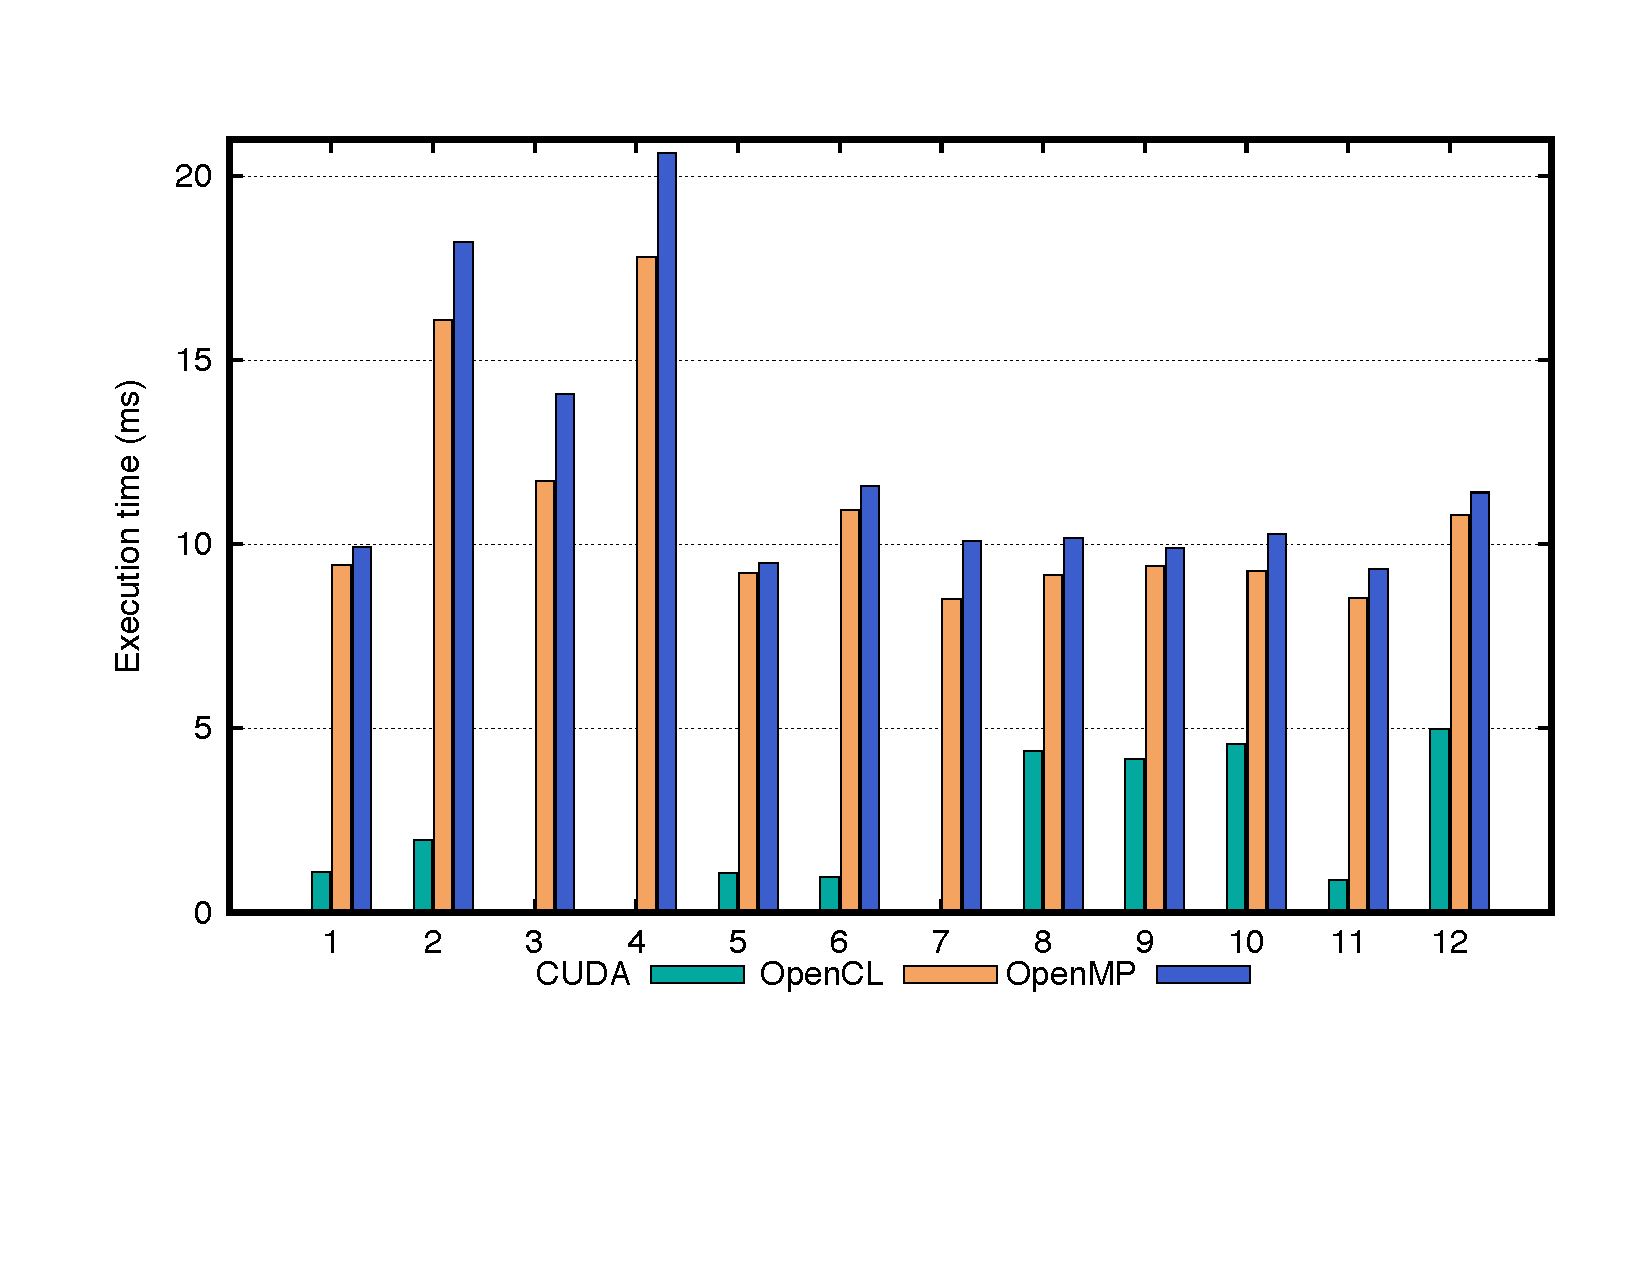
\includegraphics[scale=0.36]{images/bench_tesla.pdf}\label{fig:bench_tesla}
	}
	\vfill
	\subfloat[The execution  on Intel Core i5 with Intel Iris GPU]{
		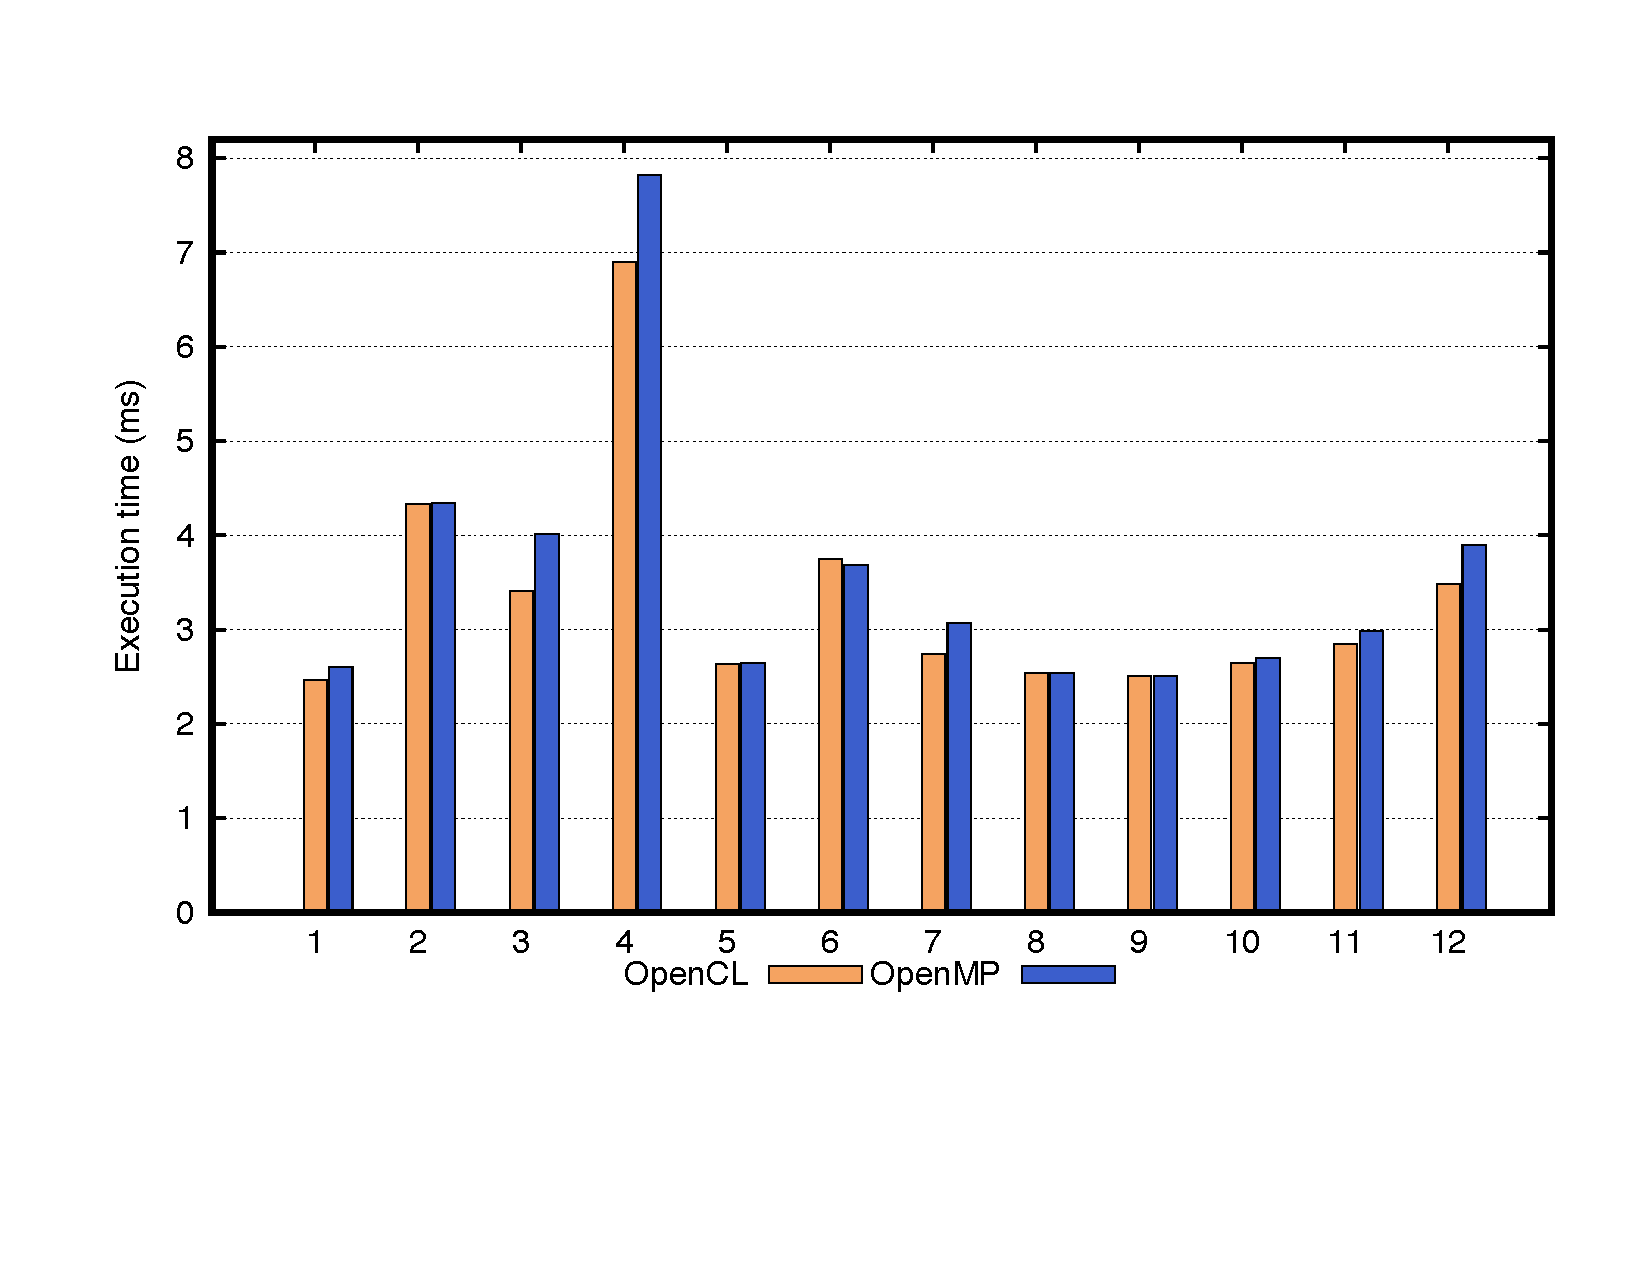
\includegraphics[scale=0.36]{images/bench_iris.pdf}\label{fig:bench_iris}
	}
	\vfill
	\subfloat[The execution  on Exynos 8890 Octa-core with ARM/Mali-T880]{
		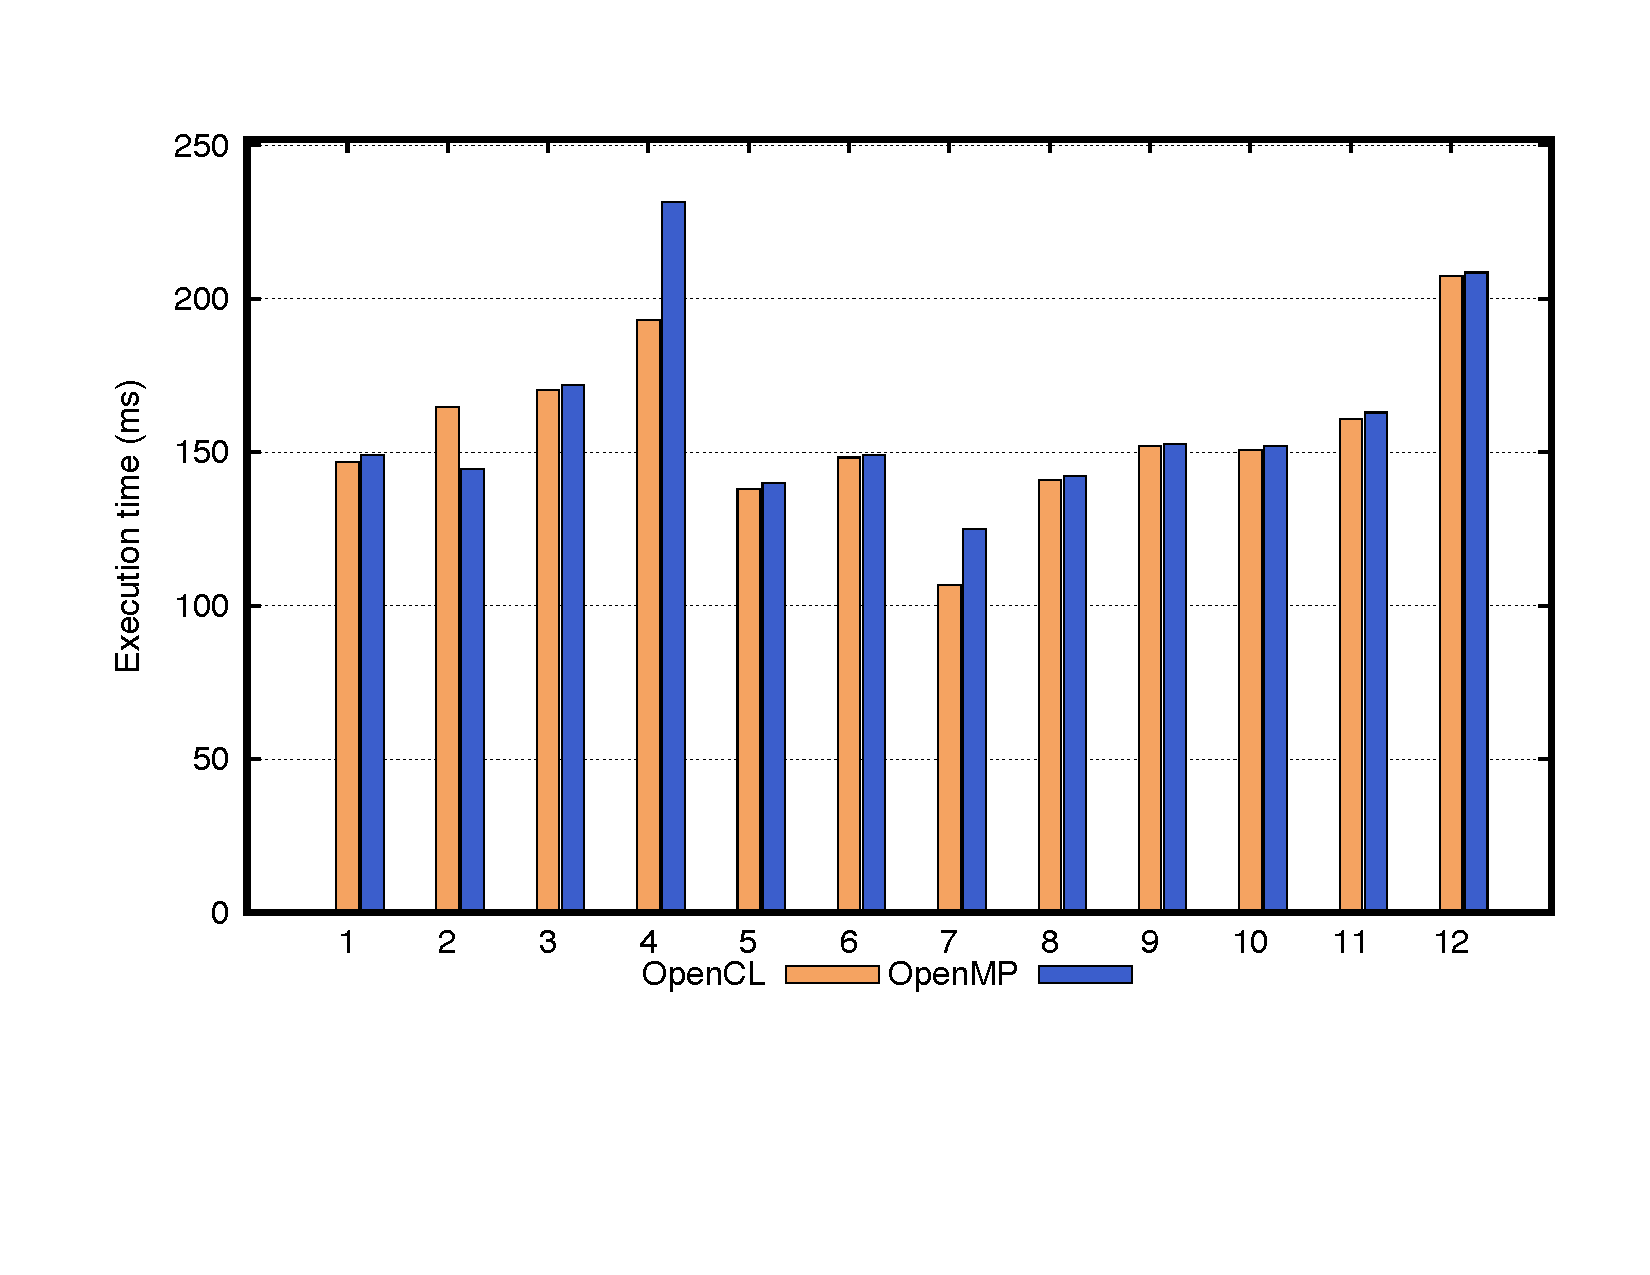
\includegraphics[scale=0.36]{images/bench_mali.pdf}\label{fig:bench_mali}
	}
\end{figure}

To evaluate the  performance of the implementation of the
proposed  OpenMP  scan clause,  three experiments  were performed.
In first  hardware  platform (NVIDIA Tesla) three    versions  of
parallel scan were tested for each benchmark program: (i) CUDA; (ii) OpenCL; and
(iii)  OpenMP. The other two  hardware platforms (Intel Iris and ARM Mali) do not
support (CUDA) and thus only the OpenCL    and    OpenMP    implementations   were
used.

The  graphs  in~\rfign{bench_tesla}{bench_iris}{bench_mali}  display
the results.  The horizontal axis of the graphs denote the number of
the  benchmark as  in  \rtab{benchmark} and  the  vertical axis  the
execution time.   In order to  provide a  minimum fair load  for the
GPUs and  to minimize the  influence of the data  offloading latency
appropriate  data sizes  were used  for  each input  data. In  other
words,  input  sizes of  $1M$  elements  were  used for  the  NVIDIA
platform and inputs  of $512K$ elements were used for  the other two
(smaller) hardware platforms (Intel and ARM) .

The  graph  in~\rfig{bench_tesla}  do  not  show  the
results  for  the  CUDA  version  of  experiments  3  (Polynomial
Evaluation), 4 (Linear Recurrences) and 7 (Adding Big Integers) due to
the lack of support to structured inputs in the CUDA Thrust library.

As  shown in~\rfig{bench_tesla}  for all  programs the
CUDA   version   performed  much better   than   the   OpenCL  and   OpenMP
versions. This is expected, given  that the Trust library is optimized
and specialized  to NVIDIA devices.  On the  other hand, the  focus of
this work is to enable a generic scan implementation that could run on
a  broad range  of  heterogeneous  devices  and  not only  NVIDIA  devices.
For this  reason,  our implementation synthesizes generic OpenCL.
Of course this does not preclude us from synthesizing CUDA in the future.

In order to better compare the performance of the proposed OpenMP scan
clause to the performance of OpenCL code, we measured their percentage
difference in all three hardware platforms. The experiments revealed a
maximum  20.3\%,  an average  6.2\%,  and  a standard  deviation  7.4\%
difference in  performance. This  strongly suggests that  the proposed
clause  can  result   in  a  similar  performance   as  when  directly
programming  in OpenCL  with the  advantage of  a smaller  programming
complexity.

\begin{figure}[!t]
	\caption{Analysis of the  performance difference between  the OpenCL
		and OpenMP implementations}
	\label{fig:analysis}
	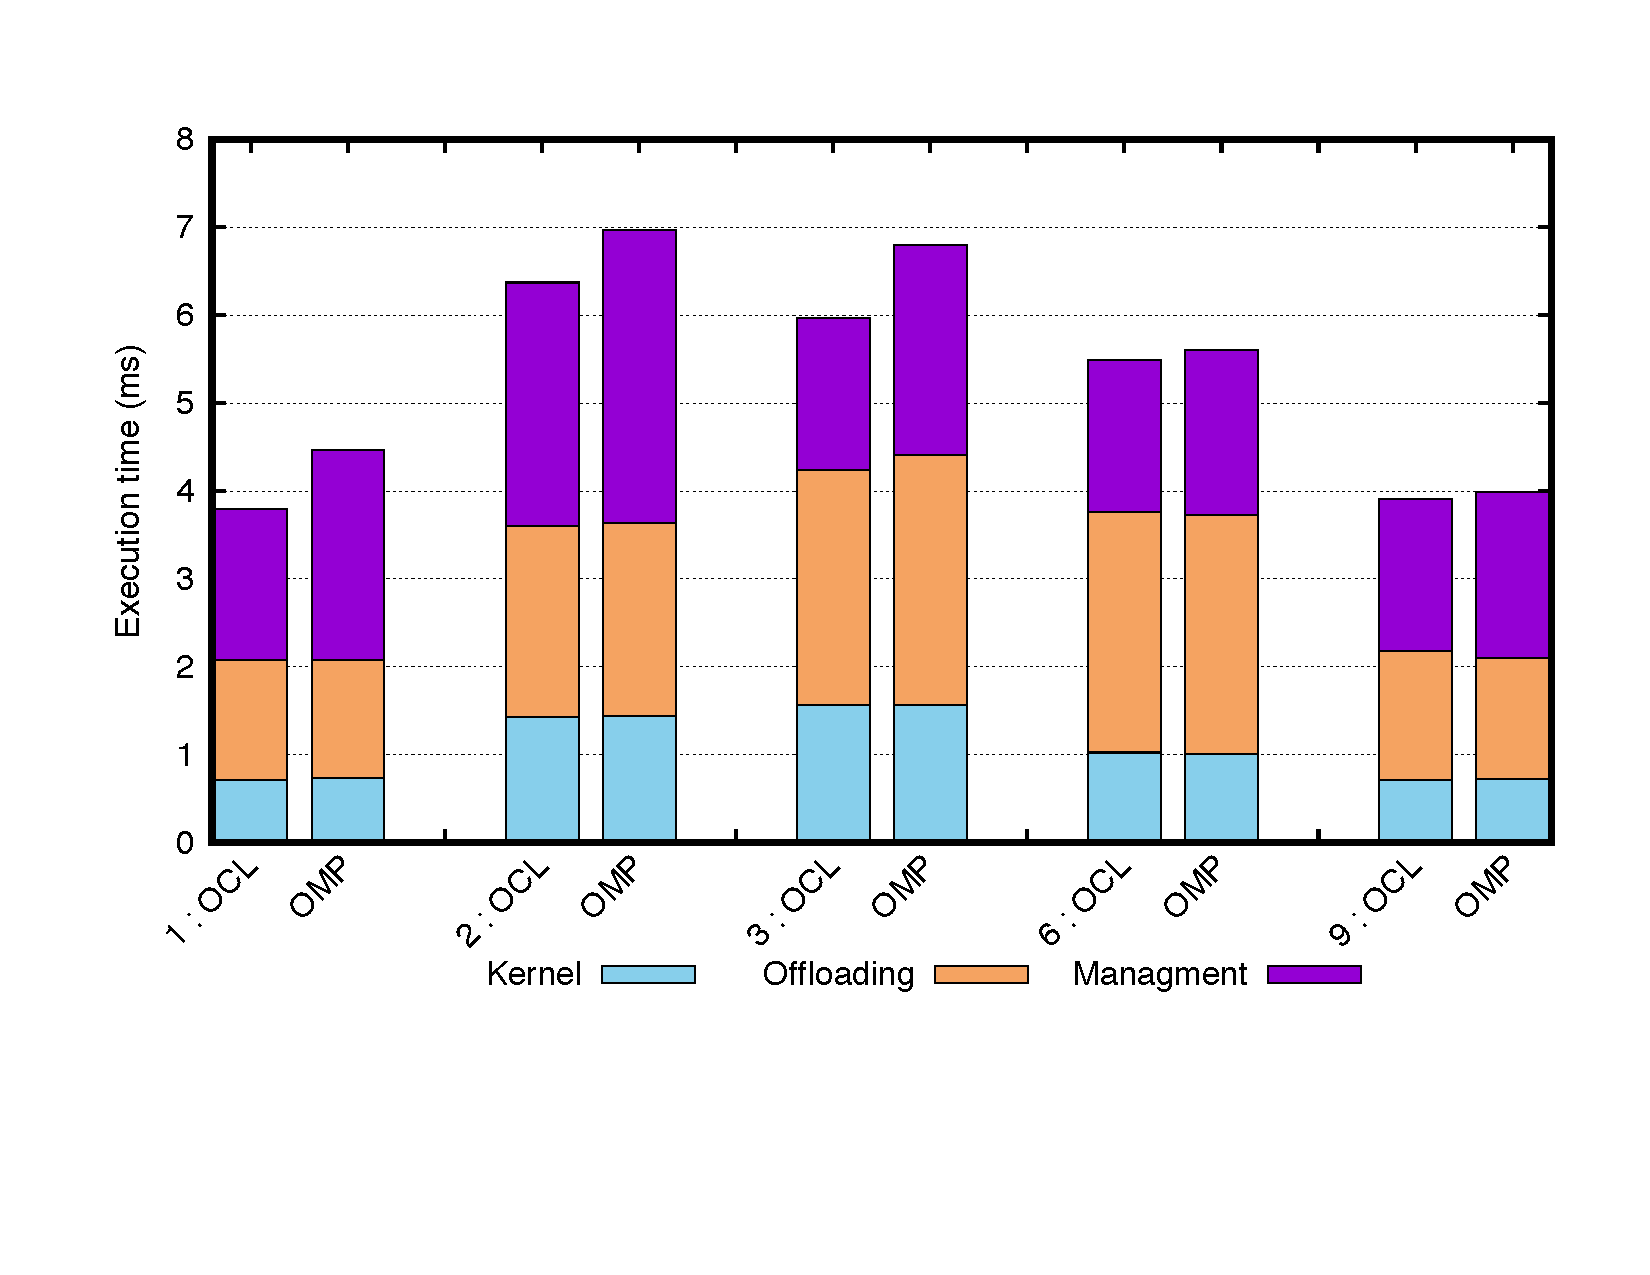
\includegraphics[scale=0.35]{images/analysis.pdf}
\end{figure}

Although small, the performance difference between the OpenCL code and
the new OpenMP  scan clause is puzzling given that  they use the exact
same   algorithm.  After a thorough analysis, we observed that the performance
difference was likely due by  the AClang runtime library.  To evaluate
that, a  new set of  experiments with profile enabled  was performed.
Figure~\ref{fig:analysis}  shows the  total  execution  time for  some
micro-benchmarks.  On the x-axis of  the figure are benchmark programs
identified by their numbers as  listed in~\ref{tab:benchmark} followed by
a label  OCL (OpenCL)  or OMP (OpenMP)  to indicate  the corresponding
implementation. On the  y-axis are program execution  times.  Each bar
in  the  figure  is  broken  down according  to  the  following  tasks
performed  during program  execution: (i)  kernel computation  (Kernel
bar);  (ii) kernel  data offloading  (Offloading bar)  and (iii)  runtime
tasks like context creation, queue management, kernel objects creation
and GPU dispatch  (Managment bar).  The analysis reveals  that 80\% to
90\% of  the slowdown over  the OpenCL  implementation are due  to the
AClang  runtime  library, not  the  algorithm  itself.  In  fact,  the
runtime library  does not  have specific routines  to handle  the scan
operation  data management.   This was  implemented using  existent
offload and dispatch operations in the library.  We believe that it is
possible  to  reduce  this  performance  difference  significantly  by
slightly adapting the runtime library  to provide routines specific to
the new scan clause.

About large inputs, the algorithm computes  of scan operator
in accordance of user's resources, it means that the algorithm will
divide the input size in slices of total threads available in the GPU,
for example if the threads available are 1M and the size of the input
is 10M, the algorithm will run 10 times slices of 1M and then will
merge the partials slices to obtain the final answer.

\chapter{Conclusions and Future Works}
\label{cap:Conclusion}

The scan operation is a simple  and powerful parallel primitive with a
broad  range  of  applications.   This  work  presented  an  efficient
implementation of a new scan clause in OpenMP which exhibts
a similar performance as direct programming in OpenCL at a much
smaller design effort. The main findings are:

\begin{itemize}
	\item It is possible to improve  the performance of the scan clause by
	providing specific routines to handle scan (and reduction) operations
	into the AClang  runtime  library.
	\item Based on the evaluated benchmarks, and after investigating the
	reasons for the differences in performance between the OpenMP and
	OpenCL versions, it is concluded that the use of the scan clause is
	perfectly acceptable due to the ease of programming given the high
	level of abstraction of OpenMP when compared to CUDA and OpenCL.
\end{itemize}




% As referências:
\bibliographystyle{plain}
\bibliography{IEEEabrv,scan}

\end{document}
